\documentclass{neus2025}

\usepackage{hyperref}
\UseRawInputEncoding

\usepackage{url}
\usepackage{booktabs}
% \usepackage{tabularx}
\usepackage{lineno}
\usepackage{array}
\usepackage{listings}
\usepackage{amssymb,amsmath}%,amsthm}       % 
\usepackage{amsfonts}      % 
\usepackage{verbatim}
\usepackage{graphicx}
\usepackage{color}
\usepackage{tikz}
\usetikzlibrary{patterns}
\usetikzlibrary{calc}
% \usetikzlibrary{arrows,positioning,shapes,fit,calc}
% \usepackage{smartdiagram}
\usepackage{algorithm}
\usepackage[noend]{algorithmic}


% \newtheorem{corollary}{Corollary}
% \newtheorem{proposition}{Proposition}
% \newtheorem{lemma}{Lemma}
% \newtheorem{theorem}{Theorem}
% \newtheorem{definition}{Definition}
% \newtheorem{remark}{Remark}

\newcommand{\jewell}[1]{\textcolor{orange}{[Jewell: #1]}}
\newcommand{\steve}[1]{\textcolor{purple}{[Steve: #1]}}

% Padded convex hull via https://tex.stackexchange.com/a/28537
\newcommand{\convexpath}[2]{
  [   
  create hullcoords/.code={
    \global\edef\namelist{#1}
    \foreach [count=\counter] \nodename in \namelist {
      \global\edef\numberofnodes{\counter}
      \coordinate (hullcoord\counter) at (\nodename);
    }
    \coordinate (hullcoord0) at (hullcoord\numberofnodes);
    \pgfmathtruncatemacro\lastnumber{\numberofnodes+1}
    \coordinate (hullcoord\lastnumber) at (hullcoord1);
  },
  create hullcoords
  ]
  ($(hullcoord1)!#2!-90:(hullcoord0)$)
  \foreach [
  evaluate=\currentnode as \previousnode using \currentnode-1,
  evaluate=\currentnode as \nextnode using \currentnode+1
  ] \currentnode in {1,...,\numberofnodes} {
    let \p1 = ($(hullcoord\currentnode) - (hullcoord\previousnode)$),
    \n1 = {atan2(\y1,\x1) + 90},
    \p2 = ($(hullcoord\nextnode) - (hullcoord\currentnode)$),
    \n2 = {atan2(\y2,\x2) + 90},
    \n{delta} = {Mod(\n2-\n1,360) - 360}
    in 
    {arc [start angle=\n1, delta angle=\n{delta}, radius=#2]}
    -- ($(hullcoord\nextnode)!#2!-90:(hullcoord\currentnode)$) 
  }
}

\definecolor{darkblue}{rgb}{0, 0, 0.5}
\hypersetup{colorlinks=true, citecolor=darkblue, linkcolor=darkblue, urlcolor=darkblue}

% The following packages will be automatically loaded:
% amsmath, amssymb, natbib, graphicx, url, algorithm2e


\title[Neurosymbolic AI via LLMs and coherence]{Neurosymbolic artificial intelligence via large language models and coherence-driven inference}
\usepackage{times}
% Use \Name{Author Name} to specify the name.
% If the surname contains spaces, enclose the surname
% in braces, e.g. \Name{John {Smith Jones}} similarly
% if the name has a "von" part, e.g \Name{Jane {de Winter}}.
% If the first letter in the forenames is a diacritic
% enclose the diacritic in braces, e.g. \Name{{\'E}louise Smith}

% Two authors with the same address
% \coltauthor{\Name{Steve Huntsman} \Email{steve.huntsman@cynnovative.com}\and
%  \Name{Jewell Thomas} \Email{jewell.thomas@cynnovative.com}\\
%  }%\addr Address}

% Three or more authors with the same address:
% \coltauthor{\Name{Author Name1} \Email{an1@sample.com}\\
%  \Name{Author Name2} \Email{an2@sample.com}\\
%  \Name{Author Name3} \Email{an3@sample.com}\\
%  \addr Address}

% Authors with different addresses:
\author{%
 \Name{Steve Huntsman} \Email{steve.huntsman@cynnovative.com}\\
 % \addr Address 1
 \and
 \Name{Jewell Thomas} \Email{jewell.thomas@cynnovative.com}\\
 % \addr Address 2%
}

\begin{document}

\maketitle

\begin{abstract}
  We devise an algorithm to generate sets of propositions that objectively instantiate graphs that support coherence-driven inference. We then benchmark the ability of large language models (LLMs) to reconstruct coherence graphs from (a straightforward transformation of) propositions expressed in natural language, with promising results from a single prompt to models optimized for reasoning. Combining coherence-driven inference with consistency evaluations by neural models may advance the state of the art in machine cognition.
\end{abstract}

% \begin{keywords}
%   coherence, large language model, neurosymbolic
% \end{keywords}

\section{\label{sec:introduction}Introduction}

Classical \emph{coherence-driven inference} (CDI) \citep{thagard1998coherence,thagard2002coherence,blokpoel2024theoretical} models many forms of cognition as solving a constraint satisfaction problem. In this approach, propositions and their consistency relations are encoded in a weighted graph $G$ as in Figure \ref{fig:coherenceCartoon}. Up to an irrelevant constant that varies among formulations, the \emph{coherence} of $U \subseteq V(G)$ is $-\sum_{u \in U, v \not \in U} A_{uv}$, where $A$ is the weighted adjacency matrix of $G$. (As is common in the literature, we often assume $A_{uv} \in \{\pm 1\}$ in this paper; our benchmarking approach handles this case naturally.) The problem of maximizing coherence is thus an instance for the matrix $-A$ of the $\mathbf{APX}$-complete MAX-CUT problem \citep{khot2007optimal,moore2011nature,gartner2012approximation,lee2021classifying}. The objective is to cut the most negative weights in $G$ with a bipartition into accepted (= estimated true) and rejected (= estimated false) propositions. 
\footnote{In general, context matters for assigning acceptance and rejection to a computed bipartition. The most common approach is to prioritize data. For example, direct observations and firm prior conclusions carry more weight than secondhand reports and tentative prior conclusions. See \citet{blokpoel2024theoretical} for a discussion of this point and remarks about implementing a data priority scheme in the present context. (Implementing a data priority scheme is straightforward in the more general computational context outlined in \S \ref{sec:computationGeneral}: just introduce appropriately weighted [or ``hard''] single-variable clauses into a weighted SAT instance.) A natural criterion \emph{in vacuo} is to prioritize the part of the bipartition whose induced subgraph has greater normalized internal coherence.}

% %% 
% % Optimal partitions are given up to symmetry by
% %     cfi
% %     bcfi
% %     bcefi
% %     bcefhi
% % for both the weighted and unweighted cases

% %%
% E = [1,2,-1;...
%     1,3,-1;...
%     1,4,1;...
%     2,5,1;...
%     3,4,-2;...
%     3,5,-2;...
%     3,6,1;...
%     4,5,-2;...
%     4,7,1;...
%     5,8,1;...
%     6,7,-2;...
%     6,8,-2;...
%     6,9,2;...
%     7,8,-2;...
%     7,9,-1;...
%     8,9,-1];
% src = E(:,1);
% tar = E(:,2);
% wgt = E(:,3);
% G = graph(src,tar,wgt);
% figure;
% plot(G,...
%     'XData',[0,1.732,-.866,.866,2.598,-.866,.866,2.598,0],...
%     'YData',[1,1,.5,.5,.5,-.5,-.5,-.5,-1])

% %%
% n = size(G.Nodes,1);
% pow = dec2bin(0:(2^n-1),n)-48;

% %%
% lab = char(96+(1:n));
% A = adjacency(G,'weighted');
% % A = sign(A);
% coh = zeros(size(pow,1),1);
% for j = 1:size(pow,1)
%     top = find(pow(j,:)==1);
%     bot = find(pow(j,:)==0);
%     coh(j) = sum(A(top,bot),'all');
% end
% ind = find(coh==min(coh));
% for i = 1:numel(ind)
%     disp(lab(pow(ind(i),:)~=0));
% end

\begin{figure}[htbp]
    \centering
        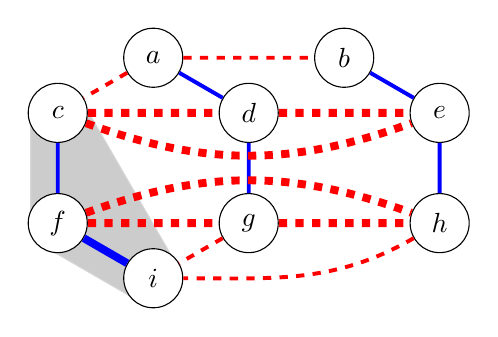
\begin{tikzpicture}[scale=1.4]
            % Draw partition first
            \coordinate (A) at (90:1);
            \coordinate (B) at (1.732,1);
            \coordinate (C) at (150:1);
            \coordinate (D) at (30:1);
            \coordinate (E) at (2.598,.5);
            \coordinate (F) at (210:1);
            \coordinate (G) at (-30:1);
            \coordinate (H) at (2.598,-.5);
            \coordinate (I) at (270:1);
            \draw[thick,black!0,fill=black,opacity=0.2] \convexpath{C,I,F}{2.5mm};
            % Label cliques
            % \node (q1) at (-.5,0) {$\top$};
            % Draw nodes
            \node [draw,circle,fill=white,minimum size=7.5mm] (a) at (A) {$a$};
            \node [draw,circle,fill=white,minimum size=7.5mm] (b) at (B) {$b$};
            \node [draw,circle,fill=white,minimum size=7.5mm] (c) at (C) {$c$};
            \node [draw,circle,fill=white,minimum size=7.5mm] (d) at (D) {$d$};
            \node [draw,circle,fill=white,minimum size=7.5mm] (e) at (E) {$e$};
            \node [draw,circle,fill=white,minimum size=7.5mm] (f) at (F) {$f$};
            \node [draw,circle,fill=white,minimum size=7.5mm] (g) at (G) {$g$};
            \node [draw,circle,fill=white,minimum size=7.5mm] (h) at (H) {$h$};
            \node [draw,circle,fill=white,minimum size=7.5mm] (i) at (I) {$i$};
            % Draw edges
            \foreach \from/\to in {
                a/d,b/e,c/f,d/g,e/h}
                \draw[line width=.5mm,blue] (\from) to (\to);
            \foreach \from/\to in {
                f/i}
                \draw[line width=1mm, blue] (\from) to (\to);
            \foreach \from/\to in {
                a/b,a/c,g/i}
                \draw[line width=.5mm,red, dashed] (\from) to (\to);
            \foreach \from/\to in {
                c/d,d/e,f/g,g/h}
                \draw[line width=1mm, red, dashed] (\from) to (\to);
            %\draw[line width=1mm, red, dashed] (c) to[out=10,in=170] (d); 
            \draw[line width=1mm, red, dashed] (c) to[out=-20,in=-160] (e); 
            % \draw[line width=1mm, red, dashed] (d) to[out=10,in=170] (e); 
            % \draw[line width=1mm, red, dashed] (f) to[out=-10,in=-170] (g); 
            \draw[line width=1mm, red, dashed] (f) to[out=20,in=160] (h); 
            %\draw[line width=1mm, red, dashed] (g) to[out=-10,in=-170] (h); 
            \draw[line width=.5mm, red, dashed] (h) to[out=-150,in=0] (i); 
        \end{tikzpicture}
        \quad
        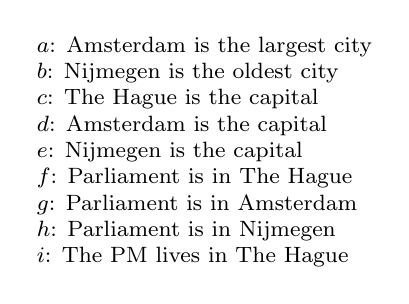
\begin{tikzpicture}
            \node[align=left,font=\footnotesize] (a) at (0,0) {
            $a$: Amsterdam is the largest city \\
            $b$: Nijmegen is the oldest city \\
            $c$: The Hague is the capital \\
            $d$: Amsterdam is the capital \\
            $e$: Nijmegen is the capital \\
            $f$: Parliament is in The Hague \\
            $g$: Parliament is in Amsterdam \\
            $h$: Parliament is in Nijmegen \\
            $i$: The PM lives in The Hague
            };
        \end{tikzpicture}
        % \begin{tikzpicture}[scale=1.67]
        %     % Draw partition first
        %     \coordinate (A) at (90:1);
        %     \coordinate (B) at (1.732,1);
        %     \coordinate (C) at (150:1);
        %     \coordinate (D) at (30:1);
        %     \coordinate (E) at (2.598,.5);
        %     \coordinate (F) at (210:1);
        %     \coordinate (G) at (-30:1);
        %     \coordinate (H) at (2.598,-.5);
        %     \coordinate (I) at (270:1);
        %     \draw[thick,black!0,fill=black,opacity=0.2] \convexpath{C,I,F}{3mm};
        %     % Label cliques
        %     % \node (q1) at (-.5,0) {$\top$};
        %     % Draw nodes
        %     \node [draw,circle,fill=white,minimum size=7.5mm] (a) at (A) {$a$};
        %     \node [draw,circle,fill=white,minimum size=7.5mm] (b) at (B) {$b$};
        %     \node [draw,circle,fill=white,minimum size=7.5mm] (c) at (C) {$c$};
        %     \node [draw,circle,fill=white,minimum size=7.5mm] (d) at (D) {$d$};
        %     \node [draw,circle,fill=white,minimum size=7.5mm] (e) at (E) {$e$};
        %     \node [draw,circle,fill=white,minimum size=7.5mm] (f) at (F) {$f$};
        %     \node [draw,circle,fill=white,minimum size=7.5mm] (g) at (G) {$g$};
        %     \node [draw,circle,fill=white,minimum size=7.5mm] (h) at (H) {$h$};
        %     \node [draw,circle,fill=white,minimum size=7.5mm] (i) at (I) {$i$};
        %     \node [align=center,text width=2cm] (a0) at (0,1.5) {\scriptsize \baselineskip=9pt Amsterdam is the largest city\par};
        %     \node [align=center,text width=2cm] (b0) at (1.732,1.5) {\scriptsize \baselineskip=9pt Nijmegen is the oldest city\par};
        %     \node [align=center,text width=2cm] (c0) at (-.866,1) {\scriptsize \baselineskip=9pt The Hague is the capital\par};
        %     \node [align=center,text width=2cm] (d0) at (.866,1) {\scriptsize \baselineskip=9pt Amsterdam is the capital\par};
        %     \node [align=center,text width=2cm] (e0) at (2.598,1) {\scriptsize \baselineskip=9pt Nijmegen is the capital\par};
        %     \node [align=center,text width=2cm] (f0) at (-.866,-1) {\scriptsize \baselineskip=9pt Parliament is in The Hague\par};
        %     \node [align=center,text width=2cm] (g0) at (.866,-1) {\scriptsize \baselineskip=9pt Parliament is in Amsterdam\par};
        %     \node [align=center,text width=2cm] (h0) at (2.598,-1) {\scriptsize \baselineskip=9pt Parliament is in Nijmegen\par};
        %     \node [align=center,text width=2cm] (h0) at (0,-1.5) {\scriptsize \baselineskip=9pt PM lives in The Hague\par};
        %     % Draw edges
        %     \foreach \from/\to in {
        %         a/d,b/e,c/f,d/g,e/h}
        %         \draw[line width=.5mm,blue] (\from) to (\to);
        %     \foreach \from/\to in {
        %         f/i}
        %         \draw[line width=1mm, blue] (\from) to (\to);
        %     \foreach \from/\to in {
        %         a/b,a/c,g/i}
        %         \draw[line width=.5mm,red, dashed] (\from) to (\to);
        %     \foreach \from/\to in {
        %         c/d,d/e,f/g,g/h}
        %         \draw[line width=1mm, red, dashed] (\from) to (\to);
        %     %\draw[line width=1mm, red, dashed] (c) to[out=10,in=170] (d); 
        %     \draw[line width=1mm, red, dashed] (c) to[out=-20,in=-160] (e); 
        %     % \draw[line width=1mm, red, dashed] (d) to[out=10,in=170] (e); 
        %     % \draw[line width=1mm, red, dashed] (f) to[out=-10,in=-170] (g); 
        %     \draw[line width=1mm, red, dashed] (f) to[out=20,in=160] (h); 
        %     %\draw[line width=1mm, red, dashed] (g) to[out=-10,in=-170] (h); 
        %     \draw[line width=.5mm, red, dashed] (h) to[out=-150,in=0] (i); 
        % \end{tikzpicture}
    \caption{A cartoon of classical coherence, elaborating on an example in \citet{blokpoel2024theoretical}. {\color{blue}Consistent (solid blue)} and {\color{red}inconsistent (red dashed)} pairs of vertices (= propositions) respectively get {\color{blue}positive} and {\color{red}negative} weights in a coherence graph, with {\bf magnitude/thickness} indicating the strength of (in)consistency. In this example, the optimal bipartitions are defined by the sets $\{c,f,i\}$ {\color{gray}(indicated with a gray vertex cluster)}, $\{b,c,f,i\}$, $\{b,c,e,f,i\}$, and $\{b,c,e,f,h,i\}$. (It turns out in this particular example that if there are only one or two edge weight magnitudes as indicated, their relative values do not affect any meaningful results due to symmetry.) Near-optimal \emph{Rashomon} solutions \citep{semenova2022existence} such as $\{a,d,f,i\}$ can become optimal if the graph is perturbed.
}
    \label{fig:coherenceCartoon}
\end{figure}

CDI is deeply informed by cognitive science, and experimentally validated by psychological case studies, including assessments of legal reasoning \citep{holyoak1999bidirectional,simon2004third}. It is a computationally credible model for causal inference \citep{thagard2004causal} suited for making decisions about ill-structured problems \citep{frigotto2015explanatory}. Other illustrations of its capacity for high-level reasoning include reaching deliberative consensus \citep{joseph2009coherence} and solving normative inconsistencies \citep{criado2016coherence}, as well as many complementary examples cited in \citet{blokpoel2024theoretical}. CDI can also explicitly incorporate ethical considerations and provide explanations of its reasoning \citep{yilmaz2017computational}. 

However, mechanisms for automatically generating coherence graphs from natural language data have not been developed: coherence graphs have almost always been constructed manually. (A notable exception is the specialized construction of \citet{joseph2009coherence} using the deduction relation of an underlying logic.) In this paper, we show how to generate a set of propositions in natural language that objectively instantiate a specified coherence graph. 
% Along related lines, Figure \ref{fig:idealGas} shows an example of graph construction for CDI using \texttt{o1-mini} \citep{jaech2024openai}. 
We then benchmark the ability of large language models (LLMs) \citep{brown2020language} to (re)construct coherence graphs, with promising results from a single prompt to models optimized for reasoning: see Figures \ref{fig:example1}, \ref{fig:example2}, and \ref{fig:cohere_graphs}, as well as Table \ref{tab:graph_uncertainty_01312025}. Another shortcoming of classical CDI that we address in \S \ref{sec:computationGeneral} is a lack of a natural mechanism for collectively relating three or more propositions, e.g., trilemmas.

% \begin{figure}[htpb]
%     \centering
%         \begin{tikzpicture}[scale=1.0]
%             % Draw nodes
%             \node [draw,circle,fill=white,minimum size=8mm] (a) at (90:1.5) {$u$};
%             \node [draw,circle,fill=white,minimum size=8mm] (b) at (162:1.5) {$t_-$};
%             \node [draw,circle,fill=white,minimum size=8mm] (c) at (234:1.5) {$v_+$};
%             \node [draw,circle,fill=white,minimum size=8mm] (d) at (306:1.5) {$v_-$};
%             \node [draw,circle,fill=white,minimum size=8mm] (e) at (18:1.5) {$t_+$};
%             % Draw edges
%             \foreach \from/\to in {
%                 a/b,a/c,a/d,a/e,b/d,c/e}
%                 \draw[ultra thick, blue] (\from) to (\to);
%             \foreach \from/\to in {
%                 b/c,b/e,c/d,d/e}
%                 \draw[ultra thick, red, dashed] (\from) to (\to);
%         \end{tikzpicture}
%         \quad        
%         \begin{tikzpicture}[scale=1.0]
%             % Draw nodes
%             \node [draw,circle,fill=white,minimum size=8mm] (a) at (90:1.5) {$u'$};
%             \node [draw,circle,fill=white,minimum size=8mm] (b) at (162:1.5) {$t_-$};
%             \node [draw,circle,fill=white,minimum size=8mm] (c) at (234:1.5) {$v_+$};
%             \node [draw,circle,fill=white,minimum size=8mm] (d) at (306:1.5) {$v_-$};
%             \node [draw,circle,fill=white,minimum size=8mm] (e) at (18:1.5) {$t_+$};
%             % Draw edges
%             \foreach \from/\to in {
%                 a/b,a/c,a/d,a/e,b/c,d/e}
%                 \draw[ultra thick, blue] (\from) to (\to);
%             \foreach \from/\to in {
%                 b/d,b/e,c/d,c/e}
%                 \draw[ultra thick, red, dashed] (\from) to (\to);
%         \end{tikzpicture}
%         \quad
%         \begin{tikzpicture}
%             \node[align=left] (a) at (0,0) {$u$: For all $q$, volume is {\bf proportional} \\ \quad to temperature. \\
%             $u'$: For all $q$, volume is {\bf inversely} \\ \quad {\bf proportional} to temperature. \\
%             $t_-$: $q$ temperature decreases. \\
%             $t_+$: $q$ temperature increases. \\
%             $v_+$: $q$ increases in volume. \\
%             $v_-$: $q$ decreases in volume. \\
%             };
%         \end{tikzpicture}
%     \caption{
%     Left: a coherence graph relating to the ideal gas law $V \propto T$, as in \citet{thagard1989explanatory}. Right: a coherence graph relating to a notional law $V \propto 1/T$. Both of these coherence graphs were readily compiled by \texttt{o1-mini} using the techniques detailed in this paper.
%     }
%     \label{fig:idealGas}
% \end{figure}

A hybrid architecture combining LLMs and CDI naturally separates concerns and is unique in the breadth of straightforward applications. CDI is suited for ``slow'' or ``system 2'' reasoning with hard computations performed on impoverished representations \citep{kahneman2011thinking}. In contrast, previous neurosymbolic  \citep{sarker2022neuro,marra2024statistical} efforts that use LLMs to help with graph coloring \citep{khandelwal2024neurosymbolic} or transform natural language data into a logical formula that can be passed to a solver  \citep{olausson2023linc,pan2023logic,ye2024satlm} reason at a low level of abstraction, cannot resolve ambiguity after the representational process, and can suffer from parsing errors \citep{feng2024language}. Meanwhile, benchmarks appropriate for evaluating the performance of such efforts using propositional or first-order logic \citep{zhong2021ar,han2022folio,saparov2023language} are not suitable for evaluating coherence.  

Meanwhile, transformer-based architectures \citep{vaswani2017attention} like LLMs are suited for ``fast'' or ``system 1'' reasoning with easy computations on rich representations \citep{lenat2023getting,bengio2024machine}. Transformers are computationally weak without chain-of-thought (CoT) reasoning, but become more powerful with it \citep{merrill2024expressive}. In principle, using CoT linear in input size allows transformers to simulate automata and recognize regular languages, or emulate a probabilistic Turing machine in quasi-quadratic time \citep{perez2021attention, nowak2024representational}. Transformers using polynomial-size CoT can also solve the problems in $\mathbf{P}$. However, the computation of a transformer with $L$ layers on a prompt of length $n$ can be performed using $O(L \log n)$ bits of memory under common assumptions. As a corollary, multilayer transformers cannot scalably solve the easy problems 2-SAT or Horn-SAT unless $\mathbf{L} = \mathbf{NL}$ \citep{peng2024limitations}. On the other hand, the representational power of multi-head transformer architectures is bounded \emph{below} by $n$-gram models \citep{rajaraman2024transformers}, which perform well in practice \citep{liu2024infini}.

The paper is organized as follows. \S \ref{sec:modelingCoherenceGraphs} explains how to produce propositions that naturally correspond to a given coherence graph. \S \ref{sec:experimentalSetup} outlines our experimental setup and \S \ref{sec:results} details the results of our experiments. We conclude in \S \ref{sec:conclusion}. Appendices respectively give substantial information on generalizing and computing CDI (\S \ref{sec:computation}); a case study in which \texttt{ChatGPT 4} outperformed a skilled human at assigning consistency ratings to proposition pairs (\S \ref{sec:vincennes}); ANOVA (\S \ref{sec:anova}); the effects of using different graph-theoretical algorithms in our benchmarking approach (\S \ref{sec:construction}); a preliminary mechanistic interpretation of how attention mechanisms may underlie our results (\S \ref{sec:cross_encoders}); characteristics of the graphs we generated for benchmarking (\S \ref{sec:graph_characteristics}), our prompt template (\S \ref{sec:prompt_example}), and finally an alternative fidelity characterization (\S \ref{sec:l1_norm_graph_anova}). {\bf We plan to release code and data in the coming weeks.}


\section{\label{sec:modelingCoherenceGraphs}Modeling coherence graphs}

Classical CDI  focuses on signed graphs, which approximate more elaborate constructions such as weighted simplicial complexes that may be appropriate for modeling and computing coherence in full generality (for which see \citet{huntsman2024prospects} and \S \ref{sec:computationGeneral}). 

{\definition Recall that a \emph{signed graph} $G_\sigma = (V,E,\sigma)$ is an undirected graph $G = (V,E)$ augmented with a \emph{sign map} $\sigma: E \rightarrow \{\pm 1\}$. A \emph{coherence graph} is a signed graph whose vertices are propositions. 
\footnote{
In practice we can use a more expressive framework than (natural language generation applied to) propositional logic, but we use the term \emph{proposition} throughout; Algorithm \ref{alg:ModelCoherenceGraph} involves \emph{bona fide} propositional formulas.
}
Two propositions $v$ and $w$ are \emph{dependent} in $G_\sigma$ if $(v,w) \in E$ (in particular, $v$ and $w$ are assumed to be distinct). Two dependent propositions are \emph{consistent for $\sigma$} (resp., \emph{inconsistent for $\sigma$}) if $\sigma(v,w) = +1$ (resp., $-1$). The left panel of Figure \ref{fig:variables} shows an example.}

\begin{figure}[htbp]
    \centering
        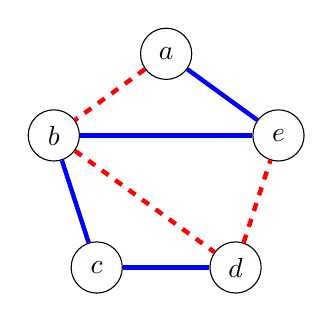
\begin{tikzpicture}[scale=1.0]
            % Draw nodes
            \node [draw,circle,fill=white,minimum size=6.5mm] (a) at (90:1.5) {$a$};
            \node [draw,circle,fill=white,minimum size=6.5mm] (b) at (162:1.5) {$b$};
            \node [draw,circle,fill=white,minimum size=6.5mm] (c) at (234:1.5) {$c$};
            \node [draw,circle,fill=white,minimum size=6.5mm] (d) at (306:1.5) {$d$};
            \node [draw,circle,fill=white,minimum size=6.5mm] (e) at (18:1.5) {$e$};
            % Draw edges
            \foreach \from/\to in {
                a/e,b/c,b/e,c/d}
                \draw[ultra thick, blue] (\from) to (\to);
            \foreach \from/\to in {
                a/b,b/d,d/e}
                \draw[ultra thick, red, dashed] (\from) to (\to);
        \end{tikzpicture}
        \quad        
        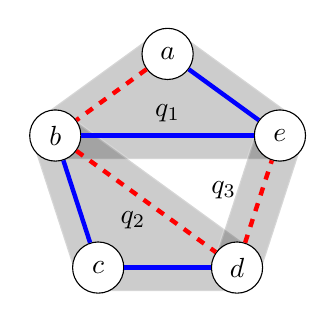
\begin{tikzpicture}[scale=1.0]
            % Draw cliques first
            \coordinate (A) at (90:1.5);
            \coordinate (B) at (162:1.5);
            \coordinate (C) at (234:1.5);
            \coordinate (D) at (306:1.5);
            \coordinate (E) at (18:1.5);
            \draw[thick,black!0,fill=black,opacity=0.2] \convexpath{A,E,B}{3mm};
            \draw[thick,black!0,fill=black,opacity=0.2] \convexpath{B,D,C}{3mm};
            \draw[thick,black!0,fill=black,opacity=0.2] \convexpath{E,D}{3mm};
            % Label cliques
            \node (q1) at (90:.75) {$q_1$};
            \node (q2) at (234:.75) {$q_2$};
            \node (q3) at (342:.75) {$q_3$};
            % Draw nodes
            \node [draw,circle,fill=white,minimum size=6.5mm] (a) at (A) {$a$};
            \node [draw,circle,fill=white,minimum size=6.5mm] (b) at (B) {$b$};
            \node [draw,circle,fill=white,minimum size=6.5mm] (c) at (C) {$c$};
            \node [draw,circle,fill=white,minimum size=6.5mm] (d) at (D) {$d$};
            \node [draw,circle,fill=white,minimum size=6.5mm] (e) at (E) {$e$};
            % Draw edges
            \foreach \from/\to in {
                a/e,b/c,b/e,c/d}
                \draw[ultra thick, blue] (\from) to (\to);
            \foreach \from/\to in {
                a/b,b/d,d/e}
                \draw[ultra thick, red, dashed] (\from) to (\to);
        \end{tikzpicture}
        \quad
        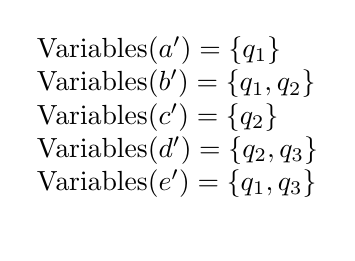
\begin{tikzpicture}
            \node[align=left] (a) at (0,0) {$\text{Variables}(a') = \{q_1\}$ \\
            $\text{Variables}(b') = \{q_1,q_2\}$ \\
            $\text{Variables}(c') = \{q_2\}$ \\
            $\text{Variables}(d') = \{q_2,q_3\}$ \\
            $\text{Variables}(e') = \{q_1,q_3\}$ \\
            };
        \end{tikzpicture}
    \caption{
    Left: a coherence graph for five propositions $\{a,\dots,e\}$, such that the pairs {\color{blue}$(a,e)$, $(b,c)$, $(b,e)$, and $(c,d)$ are consistent (indicated by solid blue edges, and corresponding to edge weights of $+1$)}; meanwhile, the pairs {\color{red}$(a,b)$, $(b,d)$, and $(d,e)$ are inconsistent (indicated by dashed red edges, and corresponding to edge weights of $-1$)}. Center: {\color{gray}cliques $q_1$, $q_2$, and $q_3$ (indicated by gray vertex clusters)} yield a minimal clique edge partition (hence cover). Right: each vertex is assigned variables corresponding to the cliques that cover it.
    }
    \label{fig:variables}
\end{figure}

A \emph{consistency oracle} $\varepsilon$ is a function that sends any pair of distinct propositions expressed in natural language to $\{-1,0,1\}$. When $\varepsilon(v,w) = -1$, $0$, and $1$, $v$ and $w$ are respectively \emph{(dependent and) inconsistent for $\varepsilon$}, \emph{independent for $\varepsilon$}, and \emph{(dependent and) consistent for $\varepsilon$}. While LLMs can effectively detect inconsistencies between two propositions (see \citet{huntsman2024prospects,kumar2024nlp}, and \S \ref{sec:vincennes}), we will initially restrict consideration  to synthetic propositions for which the output of any ``reasonable'' consistency oracle (i.e., one in which propositions that express logical formulas in natural language are evaluated in the natural way suggested by the underlying formulas) is practically obvious and unambiguous.

{\definition Given a consistency oracle $\varepsilon$, a coherence graph $G_\sigma = (V,E,\sigma)$, a set of propositions $V'$ expressed in natural language, and a bijection $\iota : V' \rightarrow V$, we say that $V'$ \emph{models $G_\sigma$ relative to $\varepsilon$} and write $V' \models_\varepsilon G_\sigma$ if for all distinct $v', w' \in V'$ we have $\varepsilon(v',w') = \sigma_0(\iota(v'),\iota(w'))$, where $\sigma_0$ extends $\sigma$ to all pairs of distinct propositions in $V$ by taking the value zero on independent pairs.}

We will give a general method for constructing $V' \models_\varepsilon G_\sigma$ under any reasonable consistency oracle $\varepsilon$, which we informally write $V' \models G_\sigma$. 

For example, taking $G_\sigma$ to be the coherence graph in the left panel of Figure \ref{fig:variables}, 
\begin{multline*}
V' = \{a': (q_1 \text{ is } p_1), \quad b': (q_1 \text{ is NOT } p_1 \text{ AND } q_2 \text{ is NOT } p_1), \quad c': (q_2 \text{ is } p_2), \\
d': (q_2 \text{ is } p_1 \text{ AND } q_3 \text{ is } p_1), \quad e': (q_1 \text{ is } p_2 \text{ AND } q_3 \text{ is NOT } p_1)\}
\end{multline*}
where the \emph{(clique) variables} $q_j$ are placeholders for nouns and the \emph{properties} $p_k$ are placeholders for gradable (hence negatable) adjectives (e.g., ``hot,'' ``bright,'' ``loud,'' etc.) and $\iota : a' \mapsto a, \dots, e' \mapsto e$, we can see that $V' \models G_\sigma$. 
A structurally equivalent model $V'' \models G_\sigma$ is
\begin{multline*}
  V'' = \{ a'': (\text{the living room is hot}), \quad
  b'': (\text{the living room is cold and the kitchen is cold}), \\
  c'': (\text{the kitchen is bright}), \quad
  d'': (\text{the kitchen is hot and the bedroom is hot}), \\
  e'': (\text{the living room is bright and the bedroom is cold}) \}.
\end{multline*}
% \begin{align*}
%   V'' = \{ a'': & \ (\text{the living room is hot}), \\
%   b'': & \ (\text{the living room is cold and the kitchen is cold}), \\
%   c'': & \ (\text{the kitchen is bright}), \\
%   d'': & \ (\text{the kitchen is hot and the bedroom is hot}), \\
%   e'': & \ (\text{the living room is bright and the bedroom is cold}) \}.
% \end{align*}
While there are structurally inequivalent sets of propositions that model $G_\sigma$, a set of the form above is extremal in that its clique edge cover and star forest decomposition are minimal: see \S \ref{sec:basicModel}. 


\subsection{\label{sec:basicModel}An algorithm for modeling coherence graphs}

Here we detail how to construct a set of propositions that model a coherence graph.

{\definition A \emph{clique edge cover} of a graph $G$ \citep{erdos1966representation,gross2018graph,conte2020large} is a set of cliques in $G$ whose edges cover $E(G)$. A \emph{star forest decomposition} of $G$ \citep{akiyama1985factors,kottarathil2024graph} is a partition of $E(G)$ into star forests, i.e., forests whose connected components each have only a single vertex of degree greater than 1: see Figure \ref{fig:properties}.}

\begin{figure}[htbp]
    \centering
        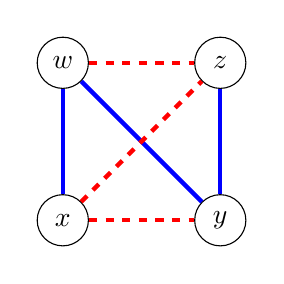
\begin{tikzpicture}[scale=1.0]
            % Draw star forests first
            \coordinate (W) at (-1,1);
            \coordinate (X) at (-1,-1);
            \coordinate (Y) at (1,-1);
            \coordinate (Z) at (1,1);
            \draw[black!0,pattern color=white,pattern=north east lines] \convexpath{W,Z}{4mm};
            \draw[black!0,pattern color=white,pattern=north west lines] \convexpath{X,Y}{4mm};
            \draw[black!0,pattern color=white,pattern=horizontal lines] \convexpath{X,Z}{4mm};
            % Draw nodes
            \node [draw,circle,fill=white,minimum size=6.5mm] (w) at (-1,1) {$w$};
            \node [draw,circle,fill=white,minimum size=6.5mm] (x) at (-1,-1) {$x$};
            \node [draw,circle,fill=white,minimum size=6.5mm] (y) at (1,-1) {$y$};
            \node [draw,circle,fill=white,minimum size=6.5mm] (z) at (1,1) {$z$};
            % Draw edges
            \foreach \from/\to in {
                w/x,w/y,y/z}
                \draw[ultra thick, blue] (\from) to (\to);
            \foreach \from/\to in {
                w/z,x/y,x/z}
                \draw[ultra thick, red, dashed] (\from) to (\to);
        \end{tikzpicture}
        \quad
        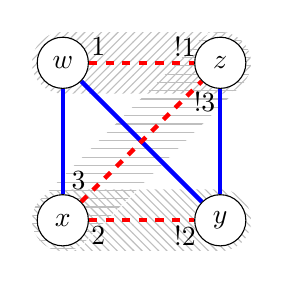
\begin{tikzpicture}[scale=1.0]
            % Draw star forests first
            \coordinate (W) at (-1,1);
            \coordinate (X) at (-1,-1);
            \coordinate (Y) at (1,-1);
            \coordinate (Z) at (1,1);
            \draw[black!0,pattern color=lightgray,pattern=north east lines] \convexpath{W,Z}{4mm};
            \draw[black!0,pattern color=lightgray,pattern=north west lines] \convexpath{X,Y}{4mm};
            \draw[black!0,pattern color=lightgray,pattern=horizontal lines] \convexpath{X,Z}{4mm};
            % Draw nodes
            \node [draw,circle,fill=white,minimum size=6.5mm] (w) at (-1,1) {$w$};
            \node [draw,circle,fill=white,minimum size=6.5mm] (x) at (-1,-1) {$x$};
            \node [draw,circle,fill=white,minimum size=6.5mm] (y) at (1,-1) {$y$};
            \node [draw,circle,fill=white,minimum size=6.5mm] (z) at (1,1) {$z$};
            % Draw edges
            \foreach \from/\to in {
                w/x,w/y,y/z}
                \draw[ultra thick, blue] (\from) to (\to);
            \foreach \from/\to in {
                w/z,x/y,x/z}
                \draw[ultra thick, red, dashed] (\from) to (\to);
            % Annotate star forests
            \node (A1) at (-.55,1.2) {$1$};
            \node (A0) at (.55,1.2) {$!1$};
            \node (B1) at (-.55,-1.2) {$2$};
            \node (B0) at (.55,-1.2) {$!2$};
            \node (C1) at (-.8,-.5) {$3$};
            \node (C0) at (.8,.5) {$!3$};
        \end{tikzpicture}
        \quad
        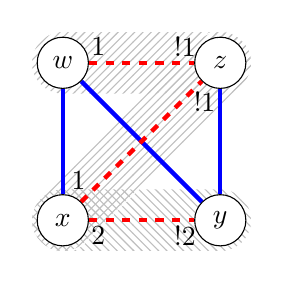
\begin{tikzpicture}[scale=1.0]
            % Draw star forests first
            \coordinate (W) at (-1,1);
            \coordinate (X) at (-1,-1);
            \coordinate (Y) at (1,-1);
            \coordinate (Z) at (1,1);
            \draw[black!0,pattern color=lightgray,pattern=north east lines] \convexpath{W,Z}{4mm};
            \draw[black!0,pattern color=lightgray,pattern=north west lines] \convexpath{X,Y}{4mm};
            \draw[black!0,pattern color=lightgray,pattern=north east lines] \convexpath{X,Z}{4mm};
            % Draw nodes
            \node [draw,circle,fill=white,minimum size=6.5mm] (w) at (-1,1) {$w$};
            \node [draw,circle,fill=white,minimum size=6.5mm] (x) at (-1,-1) {$x$};
            \node [draw,circle,fill=white,minimum size=6.5mm] (y) at (1,-1) {$y$};
            \node [draw,circle,fill=white,minimum size=6.5mm] (z) at (1,1) {$z$};
            % Draw edges
            \foreach \from/\to in {
                w/x,w/y,y/z}
                \draw[ultra thick, blue] (\from) to (\to);
            \foreach \from/\to in {
                w/z,x/y,x/z}
                \draw[ultra thick, red, dashed] (\from) to (\to);
            % Annotate star forests
            \node (A1) at (-.55,1.2) {$1$};
            \node (A0) at (.55,1.2) {$!1$};
            \node (B1) at (-.55,-1.2) {$2$};
            \node (B0) at (.55,-1.2) {$!2$};
            \node (C1) at (-.8,-.5) {$1$};
            \node (C0) at (.8,.5) {$!1$};
        \end{tikzpicture}
        \quad
        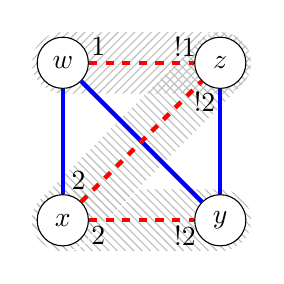
\begin{tikzpicture}[scale=1.0]
            % Draw star forests first
            \coordinate (W) at (-1,1);
            \coordinate (X) at (-1,-1);
            \coordinate (Y) at (1,-1);
            \coordinate (Z) at (1,1);
            \draw[black!0,pattern color=lightgray,pattern=north east lines] \convexpath{W,Z}{4mm};
            \draw[black!0,pattern color=lightgray,pattern=north west lines] \convexpath{X,Y}{4mm};
            \draw[black!0,pattern color=lightgray,pattern=north west lines] \convexpath{X,Z}{4mm};
            % Draw nodes
            \node [draw,circle,fill=white,minimum size=6.5mm] (w) at (-1,1) {$w$};
            \node [draw,circle,fill=white,minimum size=6.5mm] (x) at (-1,-1) {$x$};
            \node [draw,circle,fill=white,minimum size=6.5mm] (y) at (1,-1) {$y$};
            \node [draw,circle,fill=white,minimum size=6.5mm] (z) at (1,1) {$z$};
            % Draw edges
            \foreach \from/\to in {
                w/x,w/y,y/z}
                \draw[ultra thick, blue] (\from) to (\to);
            \foreach \from/\to in {
                w/z,x/y,x/z}
                \draw[ultra thick, red, dashed] (\from) to (\to);
            % Annotate star forests
            \node (A1) at (-.55,1.2) {$1$};
            \node (A0) at (.55,1.2) {$!1$};
            \node (B1) at (-.55,-1.2) {$2$};
            \node (B0) at (.55,-1.2) {$!2$};
            \node (C1) at (-.8,-.5) {$2$};
            \node (C0) at (.8,.5) {$!2$};
        \end{tikzpicture}
    \caption{
    Left: a clique in a larger notional coherence graph. Center left: the degenerate star forest decomposition of negative edges yields the greatest number of corresponding properties. The notations $n$ and $!n$ respectively indicate inconsistent propositional clauses of the form $(q \Rightarrow p_n)$ and $(q \Rightarrow \lnot p_n)$. For example, if $\Rightarrow p_1$, $\Rightarrow p_2$, and $\Rightarrow p_3$ respectively correspond to ``is hot,'', ``is bright,'' and ``is loud,'' then a natural language expression of modeling propositions is $\{w' : (q \text{ is hot}), \ x' : (q \text{ is bright AND loud}), \ y' : (q \text{ is dark}), \ z' : (q \text{ is cold AND quiet})\}$. Right panels: the two star forest decompositions of minimal size yield the minimal number of corresponding properties. The panel on the right corresponds to $\{w' : (q \text{ is hot}), \ x' : (q \text{ is bright}), \ y' : (q \text{ is dark}), \ z' : (q \text{ is cold AND dark})\}$. 
    }
    \label{fig:properties}
\end{figure}

Note that the sizes of clique edge covers and star forest decompositions are saturated below by the \emph{intersection number} and \emph{star arboricity}, respectively.

{\theorem Given a coherence graph $G_\sigma = (V,E,\sigma)$, Algorithm \ref{alg:ModelCoherenceGraph} produces $V' \models G_\sigma$.}

\begin{proof}
It suffices to show that $\varepsilon(v',w') = \sigma_0(\iota(v'),\iota(w'))$ via a case analysis. 

First, suppose that $\sigma_0(\iota(v'),\iota(w')) = 1$: here, we need to show that $v'$ and $w'$ are consistent. The respective formulas $\phi(\iota(v'))$ and $\phi(\iota(w'))$ only share common variables in clauses of the form $(q_j \Rightarrow p(v'))$ and $(q_j \Rightarrow p(w'))$. These formulas and their natural language expressions are both consistent unless $p(v') = \lnot p(w')$, which can only occur if $\sigma_0(\iota(v'),\iota(w')) = -1$, a contradiction.

Next, suppose that $\sigma_0(\iota(v'),\iota(w')) = 0$: here, we need to show that $v'$ and $w'$ are independent. Now $\iota(v')$ and $\iota(w')$ are not in a common clique, so the respective formulas $\phi(\iota(v'))$ and $\phi(\iota(w'))$ do not share any common variables. The required result follows.

Finally, suppose that $\sigma_0(\iota(v'),\iota(w')) = -1$: here, we need to show that $v'$ and $w'$ are inconsistent. Now the formulas $\phi(\iota(v'))$ and $\phi(\iota(w'))$ respectively contain clauses of the form $(q_j \Rightarrow p_k)$ and $(q_j \Rightarrow \lnot p_k)$ for some clique $C_j$ and star forest $F_k$ in the graph induced by $E^-_j$. Thus both the formulas and their natural language expressions are inconsistent. 
\end{proof}

\begin{algorithm}
  \caption{\textsc{ModelCoherenceGraph}$(G_\sigma)$}
  \label{alg:ModelCoherenceGraph}
\begin{algorithmic}[1]
  \REQUIRE Coherence graph $G_\sigma$ 
  \STATE Produce a clique edge cover $C = \{C_1,\dots,C_m\}$ of $G_\sigma$
  \FOR{$v \in V = V(G_\sigma)$}
    \STATE $\phi(v) \leftarrow \varnothing$ \hfill \emph{// initialize with empty propositional formula}
  \ENDFOR
  \FOR{$C_j \in C$}
    \STATE $E^-_j \leftarrow \{(v,w) \in E(C_j) : \sigma(v,w) = -1\}$
    \STATE Produce a star forest decomposition $F = \{F_1,\dots,F_n\}$ of the graph induced by $E^-_j$
    \FOR{$F_k \in F$}
      \FOR{each star $S$ in $F_k$}
        \STATE $r \leftarrow \text{root of } S$
        \STATE $\phi(r) \leftarrow \phi(r) \land (q_j \Rightarrow p_k)$ \hfill \emph{// ``\dots AND $q_j$ has property $p_k$''}
        \FOR{each leaf vertex $\ell \in S$}
          \STATE $\phi(\ell) \leftarrow \phi(\ell) \land (q_j \Rightarrow \lnot p_k)$ \hfill \emph{// ``\dots AND $q_j$ has property NOT($p_k$)''}
        \ENDFOR
      \ENDFOR
    \ENDFOR
  \ENDFOR
  \FOR{$v \in V$}
    \IF{$\phi(v) = \varnothing$}
      \STATE $\phi(v) \leftarrow (q^*_v \Rightarrow p^*_v)$ \hfill \emph{// to avoid triviality; $q^*_v$ only appears in $\phi(v)$}
    \ENDIF
    \STATE $v' \leftarrow \text{natural language expression of } \phi(v)$ \hfill \emph{// see comments above}
    \STATE $\iota(v') \leftarrow v$
  \ENDFOR
  \ENSURE $\{\iota^{-1}(v) : v \in V\} = V' \models G_\sigma$
\end{algorithmic}
\end{algorithm}

Note that Algorithm \ref{alg:ModelCoherenceGraph} does not require a specific construction for clique edge covers or for star forest decompositions. Different constructions affect the numbers of variables and properties: see \S \ref{sec:construction} for different clique edge cover approaches. While the approach of \citet{conte2020large} gives practical linear-time performance for clique edge covers on graphs of thousands to millions of vertices, we deal with smaller graphs and we can therefore employ more pedestrian techniques:
\begin{itemize}
    \item \texttt{degenerate}: take the degenerate clique edge cover formed by individual edges; 
    \item \texttt{percolation}: find all maximal cliques, then use a constraint solver to optimize a clique edge cover (see \url{https://stackoverflow.com/a/49145938});
    \item \texttt{partition}: initialize $G' = G$, then greedily partition $E(G')$ by iteratively removing edges from the largest clique, as discussed in but avoided by \citet{conte2020large}.
\end{itemize}
Note that the first and last of these techniques actually yield a clique edge partition.

Meanwhile, practical algorithms are in shorter supply for star forest decompositions. Finding small decompositions is $\mathbf{NP}$-complete \citep{hakimi1996star}. An integer linear program for star decompositions (that must be aggregated into star forest decompositions) is described in \citep{hajebi2024parameterized}, while \citep{cicalese2021star} gives a linear time (1/2)-approximation algorithm for the largest minimum star size. Meanwhile, given an arboricity-realizing algorithm such as \citep{gabow1988forests}, we get a (1/2)-approximate star arboricity-realizing algorithm by the observation of \citep{alon1992star} that any tree can be covered by two star forests. The following techniques can be applied, though here we only use the second:
\begin{itemize}
    \item take the degenerate star forest decomposition formed by individual edges;
    \item use the (1/2)-approximate algorithm for the largest minimum star size;
    \item repeatedly generate uniformly random edge partitions \citep{stam1983generation} and test that they contain no triangles or simple paths of (edge) length 3 \citep{aider2019star}: this is a viable brute force strategy for connected components on up to about 10 vertices since the corresponding number of partitions---i.e., the Bell number $B_{10}$---is 115975.
\end{itemize}


\subsection{\label{sec:benchmark}Benchmarking coherence}

Because computing coherence amounts to solving MAX-CUT (or MAX-SAT more generally as in \S \ref{sec:computationGeneral}), benchmarking CDI is mainly a question of fidelity of coherence graph reconstruction. Runtime and approximation performance of combinatorial optimization algorithms in \S \ref{sec:computation} may become important, but at scales considered here, exact solutions are always computationally feasible. 
\footnote{
Inferring a coherence graph from a set of propositions is similar to classical natural language inference or textual entailment \citep{korman2018defining}, which involves evaluating the logical relationship between two sentences (see \S \ref{sec:cross_encoders}). However, explanatory coherence describes more general properties of individual propositions and sets of propositions in the context of theory formation. Further, coherence encompasses a range of relations that include deductive entailment but also explanatory, analogical, perceptual, conceptual, and deliberative relations \citep{thagard2002coherence}. 
}

The propositions we generate for our benchmarking process use a grammar that can represent multiple types of relations, as well as uncertainty about a given assignment (see \S \ref{sec:fuzzy_uncertainty}). We note that the specific syntax used to represent propositions in the benchmark dataset is a matter of convenience, and users of the coherence benchmarking process can represent synthetic propositions using any syntax that is suitable for their application. 

We use a ``micro'' $F_1$ score to evaluate fidelity of coherence graph reconstruction for each attempt. This accounts for class imbalance among the values in $\{-1,0,1\}$ for each entry in each synthetic adjacency matrix included in our evaluation task \citep{opitz2024closer}. % In particular, we calculate F1 micro by calculating micro precision as $\frac{\sum \text{TP}}{\sum (\text{TP} + \text{FP})}$, micro recall as $\frac{\sum \text{TP}}{\sum (\text{TP} + \text{FN})}$ where TP, FP, TN, and FP are calculated across all edge types simultaneously. We then summarize F1 micro as $\frac{2 \times \text{Micro Precision} \times \text{Micro Recall}}{\text{Micro Precision} + \text{Micro Recall}}$.
\footnote{
Another approach to gauging performance is to use a distance measure, as in \S \ref{sec:l1_norm_graph_anova}. The reconstruction of a coherence graph $G_\sigma$ is automatically of the form $G'_{\sigma'}$ where $V(G_\sigma) = V(G'_{\sigma'})$. Therefore, it is easy and appropriate to use the metric $d(G_\sigma,G'_{\sigma'}) := \|A(G_\sigma)-A(G'_{\sigma'})\|_1$, where adjacency matrices are indicated, and we permit $A(\cdot) \in [-1,1]$ here for the sake of generality. This coincides with a graph edit distance in which edge insertion and deletion costs are the absolute value of the edge weight, and in which edge substitution costs are the absolute value of the difference of edge weights. Normalizing this by $|V|\cdot(|V|-1)/2$ gives a size-independent gauge of performance.
}


\section{\label{sec:experimentalSetup}Experimental setup}

We include proprietary and open-source models intentionally designed for reasoning in our evaluation.  We refer to \texttt{o1-mini} \citep{jaech2024openai}, \texttt{QwQ-32B} \citep{qwen_team_qwq_2024}, and \texttt{Sky-T1-32B} \citep{sky_t1_2025} as large reasoning models (LRMs), following the phrasing of \citet{valmeekam2024llms} to describe models designed to generate long chains of thought at inference time. 
% Table \ref{tab:models}.  
These models have high latency and inference costs \citep{abdin2024phi}. We consider  \texttt{phi-4} \citep{abdin2024phi} a small language model (SLM). We refer to the other models in our evaluation by the more generic term LLM: \texttt{gemini-2.0-flash-exp} \citep{google_deepmind_gemini_2024}, \texttt{claude-3.5-sonnet} \citep{anthropic_claude_2024}, \texttt{gpt-4o} \citep{hurst2024gpt}, \texttt{Llama-3.3-70B} \citep{meta_llama_3_3_2024}, and \texttt{gemini-1.5-pro} \citep{pichai_hassabis_2024}. 
% The output of all models was post-processed to extract structured data for evaluation.
For all models, we performed post-processing on outputs to extract structured data for evaluation.


\subsection{\label{sec:fuzzy_uncertainty} Adding uncertainty to propositions}

To evaluate model judgments of consistency under uncertainty, we borrow from \citet{Ragin2006}. We introduce uncertainty to $p$ or $\lnot p$ by sampling from triangular fuzzy membership functions defined over the unit interval, with $1$ and $0$ respectively corresponding to $p$ and $\lnot p$. After adding uncertainty, a given $p$-assignment is syntactically represented as something like $0.619*p$, while a given $\lnot p$ assignment is syntactically represented as something like $0.346*p$. 
That is, we indicate uncertainty as in the right panels of Figures \ref{fig:example1} and \ref{fig:example2}, with results in Table \ref{tab:graph_uncertainty_01312025}: meanwhile, the prompt in \S \ref{sec:prompt_example} echoes this construction.
With $p \leftarrow \alpha*p$ and $\lnot p \leftarrow \alpha_\lnot*p$ we delineate three uncertainty regimes. The \texttt{low} regime has $\alpha \in [0.75, 1]$ and $\alpha_\lnot \in [0, 0.25]$; the \texttt{medium} regime has $\alpha \in [0.625,0.75]$ and $\alpha_\lnot \in [0.25, 0.375]$, and the \texttt{high} regime has $\alpha \in [0.5, 0.625]$ and $\alpha_\lnot \in [0.375, 0.5]$. % Note that almost surely $\alpha_\lnot \neq 1-\alpha$.

Encoding numerical uncertainty in natural language in a way that ensures accurate interpretation is complicated by individual differences in interpretation related to terms such as ``approximately,'' ``certainly,'' ``about,'' ``exactly,'' etc. \citep{Krisper2019, Ferson2015}. This presents a challenge for, e.g., communicating risks related to climate change, risks of developing complications from medical treatment, or the likelihood of a given geopolitical event in the future \citep{ICD203}. The fuzzy set method above encodes diverse qualitative statements with a consistent formalism, and is directly relevant for use with words of estimative probability \citep{ICD203, kachynskyi2019national}. 

\label{sec:evalPropositions}{
\subsection{Benchmark generation}
}
%\subsubsection{Coherence graph generation}

To instantiate our benchmark, we sample coherence graphs from an Erd\H{o}s-R\'enyi (ER) distribution. We ensure that each sample graph is fully connected by joining sampled graphs to a minimum spanning tree generated for a complete graph of equivalent size with random edge weights. 

We generate 76 graphs with $|V| \in \{5, \dots, 23\}$ and tune the ER sampling parameters to target two regimes of edge density $:= |E|/$\scalebox{.75}{$\binom{|V|}{2}$}: \texttt{sparse} has a median edge density of 0.202 and \texttt{dense} has a median edge density of 0.734. 

    %# %%
    %import pandas as pd
    %import json
    %import networkx as nx
    %from networkx.readwrite import json_graph
    %
    %# from coherebench.utils import load_problems, load_inferences # need to install coherence-benchmark if you want to pull a new example
    %
    %# def fetch_reconstuction(problem_id):
    %#     problems = pd.DataFrame(load_problems('data/data/problems.json'))
    %#     inferences = pd.DataFrame(load_inferences('data/data/inference.json'))
    %#     problem = problems[problems.problem_id==problem_id]
    %
    %#     true_graph_str = json.dumps(json_graph.node_link_data(problem['true_graph'].values[0]))
    %
    %#     inference = inferences[(inferences.problem_id==problem_id) & (inferences.model=='o1-mini')]
    %#     reconstructon_G_str = json.dumps(json_graph.node_link_data(inference['inferred_graph_high_noise'].values[0]))
    %
    %#     metadata = problem[['problem_id', 'n_variables','n_properties', 'propositions_high_noise']]
    %#     return metadata, true_graph_str, reconstructon_G_str
    %
    %# %%
    %
    %# Example 1. perfect 21 node reconstruction (0 different edges)
    %
    %problem_id1 = "41d13c14-f8ed-416e-b82b-eb3ee23f53de"
    %
    %# metadata, true_graph_str, reconstructon_G_str = fetch_reconstuction(problem_id)
    %
    %metadata1 = """                              problem_id  n_variables  n_properties
    %52  41d13c14-f8ed-416e-b82b-eb3ee23f53de           27             2"""
    %
    %propositions1 = """['Proposition(a): q₃ is 0.655*Q AND q₄ is 0.7*Q AND q₅ is 0.585*Q AND q₆ is 0.642*P',
    % 'Proposition(b): q₃ is 0.698*Q AND q₇ is 0.66*Q AND q₈ is 0.582*P AND q₉ is 0.688*P AND q₁₀ is 0.614*P',
    % 'Proposition(c): q₁₁ is 0.57*Q',
    % 'Proposition(d): q₁₂ is 0.668*Q AND q₁₃ is 0.672*P AND q₁₄ is 0.656*Q',
    % 'Proposition(e): q₁ is 0.642*Q AND q₁₅ is 0.346*P AND q₁₆ is 0.619*P',
    % 'Proposition(f): q₂ is 0.639*Q AND q₁₇ is 0.68*Q AND q₁₈ is 0.64*Q AND q₁₉ is 0.577*Q',
    % 'Proposition(g): q₁ is 0.657*P AND q₂₀ is 0.609*Q AND q₂₁ is 0.562*P',
    % 'Proposition(h): q₄ is 0.652*Q AND q₂₀ is 0.679*Q AND q₂₂ is 0.735*P',
    % 'Proposition(i): q₁ is 0.425*P AND q₂₃ is 0.646*Q',
    % 'Proposition(j): q₇ is 0.571*Q AND q₁₇ is 0.698*Q',
    % 'Proposition(k): q₂₁ is 0.41*P',
    % 'Proposition(l): q₈ is 0.398*P AND q₁₁ is 0.612*Q AND q₁₂ is 0.644*Q AND q₂₄ is 0.664*P',
    % 'Proposition(m): q₅ is 0.592*Q AND q₁₅ is 0.617*P AND q₂₄ is 0.402*P',
    % 'Proposition(n): q₂ is 0.575*Q AND q₆ is 0.378*P AND q₂₅ is 0.602*Q',
    % 'Proposition(o): q₁₈ is 0.686*Q',
    % 'Proposition(p): q₂₂ is 0.342*P AND q₂₅ is 0.607*Q',
    % 'Proposition(q): q₁₃ is 0.343*P',
    % 'Proposition(r): q₂ is 0.682*Q AND q₂₆ is 0.585*Q',
    % 'Proposition(s): q₁₄ is 0.651*Q AND q₁₆ is 0.29*P AND q₁₉ is 0.595*Q AND q₂₇ is 0.646*P',
    % 'Proposition(t): q₉ is 0.336*P AND q₂₃ is 0.681*Q AND q₂₆ is 0.699*Q AND q₂₇ is 0.393*P',
    % 'Proposition(u): q₁₀ is 0.393*P']
    %"""
    %true_graph_str1 = '{"directed": false, "multigraph": false, "graph": {}, "nodes": [{"id": "a"}, {"id": "h"}, {"id": "b"}, {"id": "n"}, {"id": "l"}, {"id": "u"}, {"id": "j"}, {"id": "c"}, {"id": "d"}, {"id": "q"}, {"id": "s"}, {"id": "e"}, {"id": "g"}, {"id": "m"}, {"id": "f"}, {"id": "o"}, {"id": "r"}, {"id": "i"}, {"id": "k"}, {"id": "p"}, {"id": "t"}], "links": [{"weight": 0, "color": "blue", "source": "a", "target": "h"}, {"weight": 0, "color": "blue", "source": "a", "target": "b"}, {"weight": 1, "color": "red", "source": "a", "target": "n"}, {"weight": 0, "color": "blue", "source": "a", "target": "m"}, {"weight": 0, "color": "blue", "source": "h", "target": "g"}, {"weight": 1, "color": "red", "source": "h", "target": "p"}, {"weight": 1, "color": "red", "source": "b", "target": "l"}, {"weight": 1, "color": "red", "source": "b", "target": "u"}, {"weight": 0, "color": "blue", "source": "b", "target": "j"}, {"weight": 1, "color": "red", "source": "b", "target": "t"}, {"weight": 0, "color": "blue", "source": "n", "target": "r"}, {"weight": 0, "color": "blue", "source": "n", "target": "f"}, {"weight": 0, "color": "blue", "source": "n", "target": "p"}, {"weight": 0, "color": "blue", "source": "l", "target": "c"}, {"weight": 1, "color": "red", "source": "l", "target": "m"}, {"weight": 0, "color": "blue", "source": "l", "target": "d"}, {"weight": 0, "color": "blue", "source": "j", "target": "f"}, {"weight": 1, "color": "red", "source": "d", "target": "q"}, {"weight": 0, "color": "blue", "source": "d", "target": "s"}, {"weight": 1, "color": "red", "source": "s", "target": "e"}, {"weight": 1, "color": "red", "source": "s", "target": "t"}, {"weight": 0, "color": "blue", "source": "s", "target": "f"}, {"weight": 0, "color": "blue", "source": "e", "target": "g"}, {"weight": 1, "color": "red", "source": "e", "target": "m"}, {"weight": 0, "color": "blue", "source": "e", "target": "i"}, {"weight": 1, "color": "red", "source": "g", "target": "i"}, {"weight": 1, "color": "red", "source": "g", "target": "k"}, {"weight": 0, "color": "blue", "source": "f", "target": "o"}, {"weight": 0, "color": "blue", "source": "f", "target": "r"}, {"weight": 0, "color": "blue", "source": "r", "target": "t"}, {"weight": 0, "color": "blue", "source": "i", "target": "t"}]}'
    %reconstructon_G_str1 = '{"directed": false, "multigraph": false, "graph": {}, "nodes": [{"id": "e"}, {"id": "g"}, {"id": "i"}, {"id": "f"}, {"id": "n"}, {"id": "r"}, {"id": "a"}, {"id": "b"}, {"id": "h"}, {"id": "m"}, {"id": "j"}, {"id": "l"}, {"id": "t"}, {"id": "u"}, {"id": "c"}, {"id": "d"}, {"id": "q"}, {"id": "s"}, {"id": "o"}, {"id": "k"}, {"id": "p"}], "links": [{"weight": 0, "color": "blue", "source": "e", "target": "g"}, {"weight": 0, "color": "blue", "source": "e", "target": "i"}, {"weight": 1, "color": "red", "source": "e", "target": "m"}, {"weight": 1, "color": "red", "source": "e", "target": "s"}, {"weight": 1, "color": "red", "source": "g", "target": "i"}, {"weight": 0, "color": "blue", "source": "g", "target": "h"}, {"weight": 1, "color": "red", "source": "g", "target": "k"}, {"weight": 0, "color": "blue", "source": "i", "target": "t"}, {"weight": 0, "color": "blue", "source": "f", "target": "n"}, {"weight": 0, "color": "blue", "source": "f", "target": "r"}, {"weight": 0, "color": "blue", "source": "f", "target": "j"}, {"weight": 0, "color": "blue", "source": "f", "target": "o"}, {"weight": 0, "color": "blue", "source": "f", "target": "s"}, {"weight": 0, "color": "blue", "source": "n", "target": "r"}, {"weight": 1, "color": "red", "source": "n", "target": "a"}, {"weight": 0, "color": "blue", "source": "n", "target": "p"}, {"weight": 0, "color": "blue", "source": "r", "target": "t"}, {"weight": 0, "color": "blue", "source": "a", "target": "b"}, {"weight": 0, "color": "blue", "source": "a", "target": "h"}, {"weight": 0, "color": "blue", "source": "a", "target": "m"}, {"weight": 0, "color": "blue", "source": "b", "target": "j"}, {"weight": 1, "color": "red", "source": "b", "target": "l"}, {"weight": 1, "color": "red", "source": "b", "target": "t"}, {"weight": 1, "color": "red", "source": "b", "target": "u"}, {"weight": 1, "color": "red", "source": "h", "target": "p"}, {"weight": 1, "color": "red", "source": "m", "target": "l"}, {"weight": 0, "color": "blue", "source": "l", "target": "c"}, {"weight": 0, "color": "blue", "source": "l", "target": "d"}, {"weight": 1, "color": "red", "source": "t", "target": "s"}, {"weight": 1, "color": "red", "source": "d", "target": "q"}, {"weight": 0, "color": "blue", "source": "d", "target": "s"}]}'
    %
    %# %%
    %true_graph1 = json_graph.node_link_graph(json.loads(true_graph_str1))
    %reconstruction_graph1 = json_graph.node_link_graph(json.loads(reconstructon_G_str1))
    %
    %nx.difference(reconstruction_graph1, true_graph1).edges # EdgeView([])
    %
    %# %%
    %# Example 2. slightly bad 23 node reconstruction (20 different edges)
    %
    %problem_id2 = "7098653e-5058-433c-b9d9-fec01ff88d3c"
    %# metadata, true_graph_str, reconstructon_G_str = fetch_reconstuction(problem_id)
    %
    %metadata2 = """
    %                              problem_id  n_variables  n_properties
    %34  7098653e-5058-433c-b9d9-fec01ff88d3c           32             2
    %"""
    %
    %propositions2 = """
    %['Proposition(a): q₁ is 0.344*P AND q₂ is 0.611*P AND q₃ is 0.595*Q AND q₄ is 0.574*Q AND q₅ is 0.548*Q',
    % 'Proposition(b): q₁₁ is 0.669*P AND q₃₀ is 0.605*Q AND q₃₂ is 0.655*P',
    % 'Proposition(c): q₆ is 0.625*Q AND q₁₄ is 0.576*P AND q₁₅ is 0.667*P AND q₃₀ is 0.311*Q AND q₃₂ is 0.36*P',
    % 'Proposition(d): q₁₄ is 0.366*P AND q₃₁ is 0.664*P',
    % 'Proposition(e): q₁₉ is 0.62*P AND q₂₀ is 0.35*P AND q₂₁ is 0.529*Q',
    % 'Proposition(f): q₂₃ is 0.509*Q AND q₂₅ is 0.622*Q AND q₂₆ is 0.294*P',
    % 'Proposition(g): q₁ is 0.655*P AND q₃₀ is 0.452*P AND q₃₁ is 0.633*P',
    % 'Proposition(h): q₄ is 0.673*Q AND q₉ is 0.583*P AND q₁₀ is 0.595*P',
    % 'Proposition(i): q₇ is 0.429*P AND q₁₈ is 0.606*Q AND q₂₀ is 0.627*P AND q₂₃ is 0.58*Q AND q₂₄ is 0.557*Q',
    % 'Proposition(j): q₁₁ is 0.338*P AND q₁₂ is 0.663*Q AND q₁₃ is 0.623*Q',
    % 'Proposition(k): q₁₀ is 0.39*P AND q₂₇ is 0.575*Q',
    % 'Proposition(l): q₁₈ is 0.729*Q AND q₃₁ is 0.351*P',
    % 'Proposition(m): q₂₁ is 0.625*Q AND q₂₅ is 0.596*Q',
    % 'Proposition(n): q₂ is 0.395*P AND q₆ is 0.575*Q AND q₇ is 0.707*P AND q₈ is 0.616*Q',
    % 'Proposition(o): q₁₆ is 0.568*Q AND q₁₉ is 0.298*P AND q₂₂ is 0.656*Q',
    % 'Proposition(p): q₃₂ is 0.415*P',
    % 'Proposition(q): q₉ is 0.286*P AND q₁₂ is 0.531*Q AND q₂₆ is 0.601*P',
    % 'Proposition(r): q₁₃ is 0.638*Q AND q₂₂ is 0.585*Q AND q₂₉ is 0.564*Q',
    % 'Proposition(s): q₈ is 0.658*Q AND q₂₈ is 0.62*Q',
    % 'Proposition(t): q₂₄ is 0.628*Q AND q₂₇ is 0.638*Q AND q₂₈ is 0.593*Q',
    % 'Proposition(u): q₃ is 0.675*Q',
    % 'Proposition(v): q₁₇ is 0.656*Q AND q₂₉ is 0.557*Q',
    % 'Proposition(w): q₅ is 0.612*Q AND q₁₅ is 0.383*P AND q₁₆ is 0.615*Q AND q₁₇ is 0.699*Q']
    %"""
    %
    %true_graph_str2 = '{"directed": false, "multigraph": false, "graph": {}, "nodes": [{"id": "a"}, {"id": "g"}, {"id": "n"}, {"id": "u"}, {"id": "h"}, {"id": "b"}, {"id": "j"}, {"id": "p"}, {"id": "c"}, {"id": "d"}, {"id": "w"}, {"id": "l"}, {"id": "e"}, {"id": "o"}, {"id": "i"}, {"id": "f"}, {"id": "m"}, {"id": "q"}, {"id": "k"}, {"id": "t"}, {"id": "r"}, {"id": "v"}, {"id": "s"}], "links": [{"weight": 1, "color": "red", "source": "a", "target": "g"}, {"weight": 1, "color": "red", "source": "a", "target": "n"}, {"weight": 0, "color": "blue", "source": "a", "target": "u"}, {"weight": 0, "color": "blue", "source": "a", "target": "h"}, {"weight": 0, "color": "blue", "source": "a", "target": "w"}, {"weight": 1, "color": "red", "source": "g", "target": "b"}, {"weight": 1, "color": "red", "source": "g", "target": "c"}, {"weight": 1, "color": "red", "source": "g", "target": "d"}, {"weight": 1, "color": "red", "source": "g", "target": "l"}, {"weight": 0, "color": "blue", "source": "n", "target": "c"}, {"weight": 1, "color": "red", "source": "n", "target": "i"}, {"weight": 0, "color": "blue", "source": "n", "target": "s"}, {"weight": 1, "color": "red", "source": "h", "target": "k"}, {"weight": 1, "color": "red", "source": "h", "target": "q"}, {"weight": 1, "color": "red", "source": "b", "target": "j"}, {"weight": 1, "color": "red", "source": "b", "target": "p"}, {"weight": 1, "color": "red", "source": "b", "target": "c"}, {"weight": 0, "color": "blue", "source": "j", "target": "r"}, {"weight": 0, "color": "blue", "source": "j", "target": "q"}, {"weight": 0, "color": "blue", "source": "p", "target": "c"}, {"weight": 1, "color": "red", "source": "c", "target": "d"}, {"weight": 1, "color": "red", "source": "c", "target": "w"}, {"weight": 1, "color": "red", "source": "d", "target": "l"}, {"weight": 0, "color": "blue", "source": "w", "target": "o"}, {"weight": 0, "color": "blue", "source": "w", "target": "v"}, {"weight": 0, "color": "blue", "source": "l", "target": "i"}, {"weight": 1, "color": "red", "source": "e", "target": "o"}, {"weight": 1, "color": "red", "source": "e", "target": "i"}, {"weight": 0, "color": "blue", "source": "e", "target": "m"}, {"weight": 0, "color": "blue", "source": "o", "target": "r"}, {"weight": 0, "color": "blue", "source": "i", "target": "f"}, {"weight": 0, "color": "blue", "source": "i", "target": "t"}, {"weight": 0, "color": "blue", "source": "f", "target": "m"}, {"weight": 1, "color": "red", "source": "f", "target": "q"}, {"weight": 0, "color": "blue", "source": "k", "target": "t"}, {"weight": 0, "color": "blue", "source": "t", "target": "s"}, {"weight": 0, "color": "blue", "source": "r", "target": "v"}]}'
    %reconstructon_G_str2 = '{"directed": false, "multigraph": false, "graph": {}, "nodes": [{"id": "a"}, {"id": "h"}, {"id": "u"}, {"id": "w"}, {"id": "e"}, {"id": "m"}, {"id": "f"}, {"id": "i"}, {"id": "l"}, {"id": "t"}, {"id": "j"}, {"id": "q"}, {"id": "r"}, {"id": "k"}, {"id": "o"}, {"id": "v"}, {"id": "s"}, {"id": "d"}, {"id": "g"}, {"id": "n"}, {"id": "b"}, {"id": "c"}, {"id": "p"}], "links": [{"weight": 0, "color": "blue", "source": "a", "target": "h"}, {"weight": 0, "color": "blue", "source": "a", "target": "u"}, {"weight": 0, "color": "blue", "source": "a", "target": "w"}, {"weight": 1, "color": "red", "source": "a", "target": "d"}, {"weight": 1, "color": "red", "source": "a", "target": "g"}, {"weight": 1, "color": "red", "source": "a", "target": "n"}, {"weight": 1, "color": "red", "source": "h", "target": "k"}, {"weight": 1, "color": "red", "source": "h", "target": "q"}, {"weight": 1, "color": "red", "source": "w", "target": "c"}, {"weight": 0, "color": "blue", "source": "e", "target": "m"}, {"weight": 1, "color": "red", "source": "e", "target": "i"}, {"weight": 1, "color": "red", "source": "e", "target": "o"}, {"weight": 0, "color": "blue", "source": "m", "target": "f"}, {"weight": 0, "color": "blue", "source": "f", "target": "i"}, {"weight": 1, "color": "red", "source": "f", "target": "n"}, {"weight": 1, "color": "red", "source": "f", "target": "q"}, {"weight": 0, "color": "blue", "source": "i", "target": "l"}, {"weight": 0, "color": "blue", "source": "i", "target": "t"}, {"weight": 1, "color": "red", "source": "i", "target": "n"}, {"weight": 1, "color": "red", "source": "l", "target": "d"}, {"weight": 1, "color": "red", "source": "l", "target": "g"}, {"weight": 0, "color": "blue", "source": "t", "target": "k"}, {"weight": 0, "color": "blue", "source": "t", "target": "s"}, {"weight": 0, "color": "blue", "source": "j", "target": "q"}, {"weight": 0, "color": "blue", "source": "j", "target": "r"}, {"weight": 1, "color": "red", "source": "j", "target": "b"}, {"weight": 0, "color": "blue", "source": "r", "target": "o"}, {"weight": 0, "color": "blue", "source": "r", "target": "v"}, {"weight": 1, "color": "red", "source": "d", "target": "c"}, {"weight": 1, "color": "red", "source": "b", "target": "c"}, {"weight": 1, "color": "red", "source": "b", "target": "p"}, {"weight": 1, "color": "red", "source": "c", "target": "p"}]}'
    %
    %# %%
    %true_graph2 = json_graph.node_link_graph(json.loads(true_graph_str2))
    %reconstruction_graph2 = json_graph.node_link_graph(json.loads(reconstructon_G_str2))
    %nx.difference(reconstruction_graph2, true_graph2).edges # EdgeView([('a', 'd'), ('f', 'n')])
    %
    %
    %# %%
    %import matplotlib.pyplot as plt
    %# Draw the graph
    %nx.draw_circular(true_graph1, with_labels=True)
    %plt.show()
    %
    %
    %# %%
    %import matplotlib.pyplot as plt
    %# Draw the graph
    %pos = nx.circular_layout(sorted(true_graph1.nodes()))
    %nx.draw(true_graph1, pos=pos, with_labels=True)
    %plt.show()
    %
    %
    %# %%
    %import json
    %import tikzplotlib
    %
    %def generate_tikz(json_data, layout):
    %    """Generates TikZ code for a graph from JSON data and a layout."""
    %
    %    graph_data = json.loads(json_data)
    %
    %    tikz_code = r"""
    %\documentclass{standalone}
    %\usepackage{tikz}
    %
    %\begin{document}
    %
    %\begin{tikzpicture}[
    %  node distance=2cm, % Adjust as needed
    %  every node/.style={circle,draw,minimum size=0.7cm,inner sep=0,outer sep=0},
    %  blue edge/.style={blue, ultra thick},
    %  red edge/.style={red, ultra thick, dashed},
    %  xscale=4, % Adjust scaling as needed
    %  yscale=4,
    %]
    %
    %% Node positions
    %"""
    %
    %    for node in graph_data["nodes"]:
    %        node_id = node["id"]
    %        x, y = layout[node_id]
    %        tikz_code += f"\\node ({node_id}) at ({x},{y}) {{${node_id}$}};\n"
    %
    %    tikz_code += "\n% Edges\n"
    %
    %    for link in graph_data["links"]:
    %        source = link["source"]
    %        target = link["target"]
    %        color = link["color"]
    %        weight = link.get("weight", 0)  # Handle missing weight
    %
    %        edge_style = "blue edge" if color == "blue" else "red edge"
    %        tikz_code += f"\\draw[{edge_style}] ({source}) -- ({target});\n"
    %
    %    tikz_code += r"""
    %\end{tikzpicture}
    %
    %\end{document}
    %"""
    %    return tikz_code
    %
    %# %%
    %# json_data = true_graph_str2
    %json_data = reconstructon_G_str2
    %# pos = nx.circular_layout(true_graph2)
    %pos = nx.circular_layout(sorted(true_graph2.nodes()))
    %
    %layout = {x: list(pos[x]) for x in pos}
    %tikz_code = generate_tikz(json_data, layout)
    %print(tikz_code)

    %# %%
    %def replace_unicode_subscript(text):
    %    """Replaces unicode subscripts with normal text equivalents."""
    %
    %    subscript_map = {
    %        "\u2080": "0",
    %        "\u2081": "1",
    %        "\u2082": "2",
    %        "\u2083": "3",
    %        "\u2084": "4",
    %        "\u2085": "5",
    %        "\u2086": "6",
    %        "\u2087": "7",
    %        "\u2088": "8",
    %        "\u2089": "9",
    %    }
    %
    %    for subscript, normal in subscript_map.items():
    %        text = text.replace(subscript, normal)
    %
    %    return text
    %
    %# %%
    %print(replace_unicode_subscript(propositions1))

\begin{figure}[htbp]
  \centering
    \resizebox{.24\textwidth}{!}{%
        % true 1
        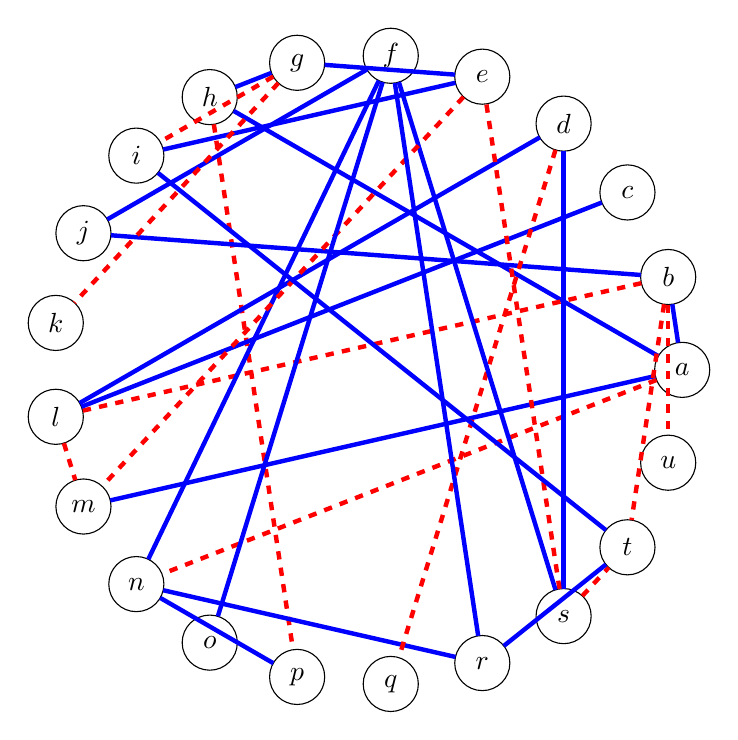
\begin{tikzpicture}[
          node distance=2cm, % Adjust as needed
          every node/.style={circle,draw,minimum size=0.7cm,inner sep=0,outer sep=0},
          blue edge/.style={blue, ultra thick},
          red edge/.style={red, ultra thick, dashed},
          xscale=4, % Adjust scaling as needed
          yscale=4,
        ]
        
        % Node positions
        \node (a) at (1.0,4.257474623792601e-09) {$a$};
        \node (h) at (-0.5000000585402762,0.8660253918837754) {$h$};
        \node (b) at (0.9555727839785156,0.29475519465920813) {$b$};
        \node (n) at (-0.7330518352608938,-0.6801727366730055) {$n$};
        \node (l) at (-0.9888308034135964,-0.14904225926382042) {$l$};
        \node (u) at (0.9555727839785156,-0.29475527555122594) {$u$};
        \node (j) at (-0.9009688483100784,0.4338838199533992) {$j$};
        \node (c) at (0.8262387515347354,0.563320104165219) {$c$};
        \node (d) at (0.6234897973824897,0.7818315066171321) {$d$};
        \node (q) at (0.07473030006975624,-0.9972037623345826) {$q$};
        \node (s) at (0.6234896185685554,-0.7818316173114723) {$s$};
        \node (e) at (0.3653409783575216,0.9308737552372659) {$e$};
        \node (g) at (-0.22252094658888455,0.9749279057873659) {$g$};
        \node (m) at (-0.9009688483100784,-0.4338837518338052) {$m$};
        \node (f) at (0.07473012125582204,0.9972037708495318) {$f$};
        \node (o) at (-0.49999990952866424,-0.8660254429734708) {$o$};
        \node (r) at (0.36534100815984394,-0.9308737467223167) {$r$};
        \node (i) at (-0.7330518948655386,0.68017268558331) {$i$};
        \node (k) at (-0.9888308034135964,0.14904232738341439) {$k$};
        \node (p) at (-0.22252100619352927,-0.9749278972724167) {$p$};
        \node (t) at (0.82623881113938,-0.5633199764409804) {$t$};
        
        % Edges
        \draw[blue edge] (a) -- (h);
        \draw[blue edge] (a) -- (b);
        \draw[red edge] (a) -- (n);
        \draw[blue edge] (a) -- (m);
        \draw[blue edge] (h) -- (g);
        \draw[red edge] (h) -- (p);
        \draw[red edge] (b) -- (l);
        \draw[red edge] (b) -- (u);
        \draw[blue edge] (b) -- (j);
        \draw[red edge] (b) -- (t);
        \draw[blue edge] (n) -- (r);
        \draw[blue edge] (n) -- (f);
        \draw[blue edge] (n) -- (p);
        \draw[blue edge] (l) -- (c);
        \draw[red edge] (l) -- (m);
        \draw[blue edge] (l) -- (d);
        \draw[blue edge] (j) -- (f);
        \draw[red edge] (d) -- (q);
        \draw[blue edge] (d) -- (s);
        \draw[red edge] (s) -- (e);
        \draw[red edge] (s) -- (t);
        \draw[blue edge] (s) -- (f);
        \draw[blue edge] (e) -- (g);
        \draw[red edge] (e) -- (m);
        \draw[blue edge] (e) -- (i);
        \draw[red edge] (g) -- (i);
        \draw[red edge] (g) -- (k);
        \draw[blue edge] (f) -- (o);
        \draw[blue edge] (f) -- (r);
        \draw[blue edge] (r) -- (t);
        \draw[blue edge] (i) -- (t);
        
        \end{tikzpicture}
    }
    \resizebox{.24\textwidth}{!}{%
        % reconstruction 1
        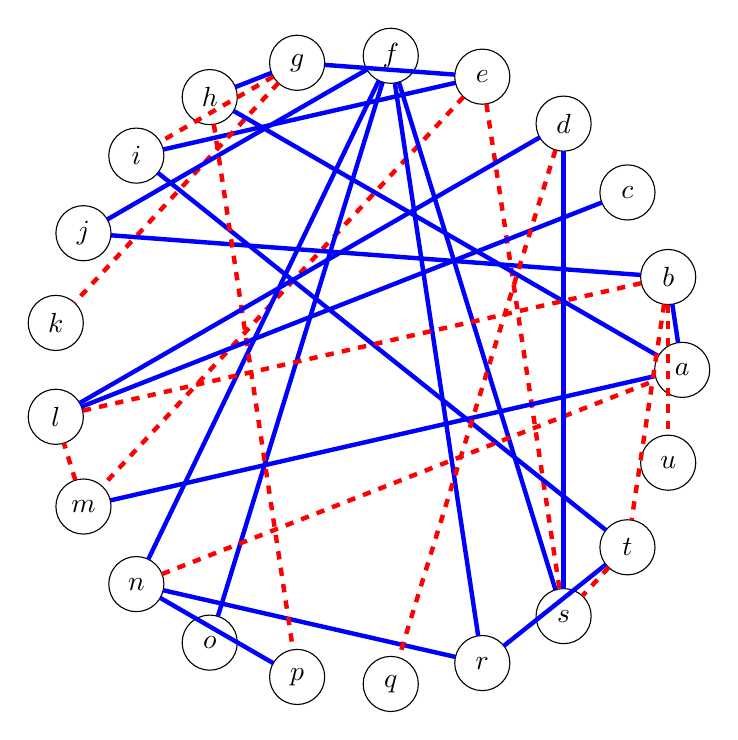
\begin{tikzpicture}[
          node distance=2cm, % Adjust as needed
          every node/.style={circle,draw,minimum size=0.7cm,inner sep=0,outer sep=0},
          blue edge/.style={blue, ultra thick},
          red edge/.style={red, ultra thick, dashed},
          xscale=4, % Adjust scaling as needed
          yscale=4,
        ]
        
        % Node positions
        \node (e) at (0.3653409783575216,0.9308737552372659) {$e$};
        \node (g) at (-0.22252094658888455,0.9749279057873659) {$g$};
        \node (i) at (-0.7330518948655386,0.68017268558331) {$i$};
        \node (f) at (0.07473012125582204,0.9972037708495318) {$f$};
        \node (n) at (-0.7330518352608938,-0.6801727366730055) {$n$};
        \node (r) at (0.36534100815984394,-0.9308737467223167) {$r$};
        \node (a) at (1.0,4.257474623792601e-09) {$a$};
        \node (b) at (0.9555727839785156,0.29475519465920813) {$b$};
        \node (h) at (-0.5000000585402762,0.8660253918837754) {$h$};
        \node (m) at (-0.9009688483100784,-0.4338837518338052) {$m$};
        \node (j) at (-0.9009688483100784,0.4338838199533992) {$j$};
        \node (l) at (-0.9888308034135964,-0.14904225926382042) {$l$};
        \node (t) at (0.82623881113938,-0.5633199764409804) {$t$};
        \node (u) at (0.9555727839785156,-0.29475527555122594) {$u$};
        \node (c) at (0.8262387515347354,0.563320104165219) {$c$};
        \node (d) at (0.6234897973824897,0.7818315066171321) {$d$};
        \node (q) at (0.07473030006975624,-0.9972037623345826) {$q$};
        \node (s) at (0.6234896185685554,-0.7818316173114723) {$s$};
        \node (o) at (-0.49999990952866424,-0.8660254429734708) {$o$};
        \node (k) at (-0.9888308034135964,0.14904232738341439) {$k$};
        \node (p) at (-0.22252100619352927,-0.9749278972724167) {$p$};
        
        % Edges
        \draw[blue edge] (e) -- (g);
        \draw[blue edge] (e) -- (i);
        \draw[red edge] (e) -- (m);
        \draw[red edge] (e) -- (s);
        \draw[red edge] (g) -- (i);
        \draw[blue edge] (g) -- (h);
        \draw[red edge] (g) -- (k);
        \draw[blue edge] (i) -- (t);
        \draw[blue edge] (f) -- (n);
        \draw[blue edge] (f) -- (r);
        \draw[blue edge] (f) -- (j);
        \draw[blue edge] (f) -- (o);
        \draw[blue edge] (f) -- (s);
        \draw[blue edge] (n) -- (r);
        \draw[red edge] (n) -- (a);
        \draw[blue edge] (n) -- (p);
        \draw[blue edge] (r) -- (t);
        \draw[blue edge] (a) -- (b);
        \draw[blue edge] (a) -- (h);
        \draw[blue edge] (a) -- (m);
        \draw[blue edge] (b) -- (j);
        \draw[red edge] (b) -- (l);
        \draw[red edge] (b) -- (t);
        \draw[red edge] (b) -- (u);
        \draw[red edge] (h) -- (p);
        \draw[red edge] (m) -- (l);
        \draw[blue edge] (l) -- (c);
        \draw[blue edge] (l) -- (d);
        \draw[red edge] (t) -- (s);
        \draw[red edge] (d) -- (q);
        \draw[blue edge] (d) -- (s);
        
        \end{tikzpicture}
    }
    \resizebox{.49\textwidth}{!}{%
        % true 2
        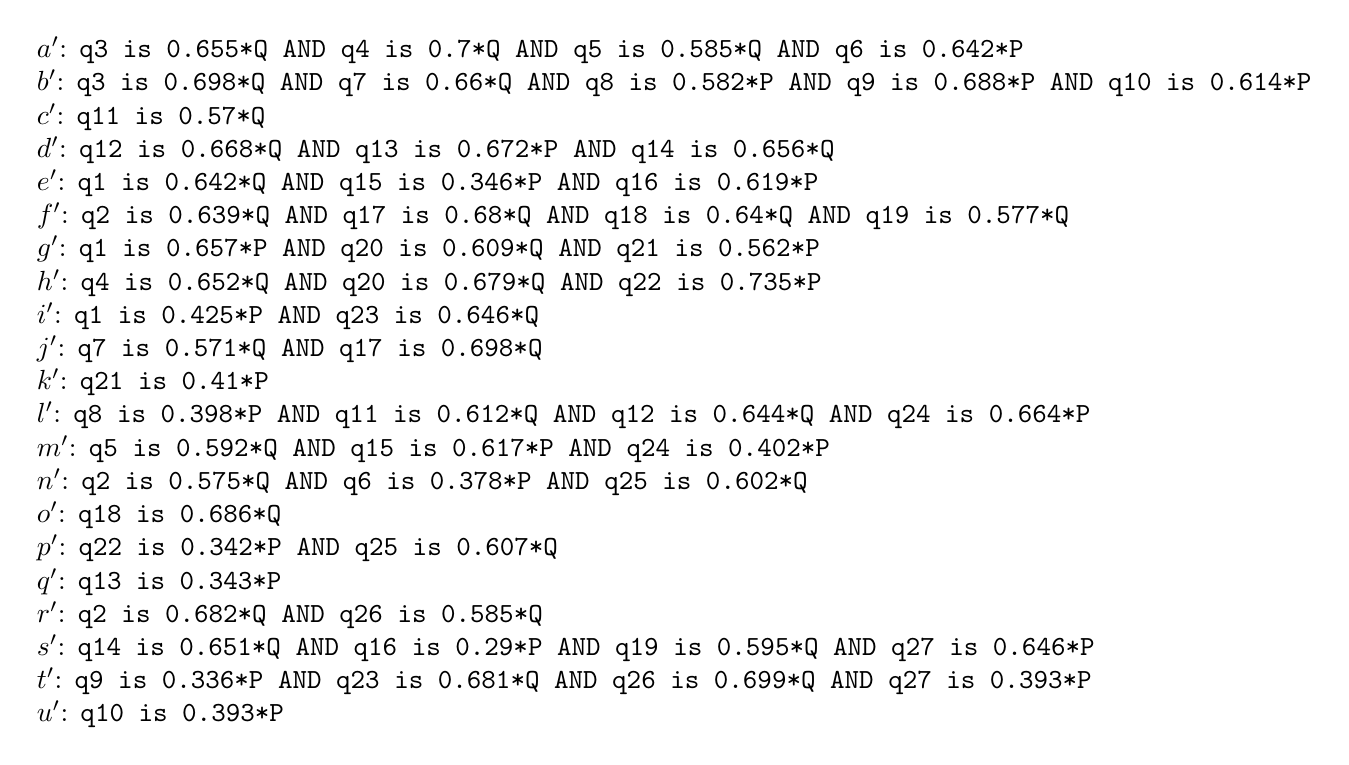
\begin{tikzpicture}[
          xscale=4, % Adjust scaling as needed
          yscale=4,
        ]
            \node[align=left] (a) at (0,0) {
                $a'$: \texttt{q3 is 0.655*Q AND q4 is 0.7*Q AND q5 is 0.585*Q AND q6 is 0.642*P} \\
                $b'$: \texttt{q3 is 0.698*Q AND q7 is 0.66*Q AND q8 is 0.582*P AND q9 is 0.688*P AND q10 is 0.614*P} \\
                $c'$: \texttt{q11 is 0.57*Q} \\
                $d'$: \texttt{q12 is 0.668*Q AND q13 is 0.672*P AND q14 is 0.656*Q} \\
                $e'$: \texttt{q1 is 0.642*Q AND q15 is 0.346*P AND q16 is 0.619*P} \\
                $f'$: \texttt{q2 is 0.639*Q AND q17 is 0.68*Q AND q18 is 0.64*Q AND q19 is 0.577*Q} \\
                $g'$: \texttt{q1 is 0.657*P AND q20 is 0.609*Q AND q21 is 0.562*P} \\
                $h'$: \texttt{q4 is 0.652*Q AND q20 is 0.679*Q AND q22 is 0.735*P} \\
                $i'$: \texttt{q1 is 0.425*P AND q23 is 0.646*Q} \\
                $j'$: \texttt{q7 is 0.571*Q AND q17 is 0.698*Q} \\
                $k'$: \texttt{q21 is 0.41*P} \\
                $l'$: \texttt{q8 is 0.398*P AND q11 is 0.612*Q AND q12 is 0.644*Q AND q24 is 0.664*P} \\
                $m'$: \texttt{q5 is 0.592*Q AND q15 is 0.617*P AND q24 is 0.402*P} \\
                $n'$: \texttt{q2 is 0.575*Q AND q6 is 0.378*P AND q25 is 0.602*Q} \\
                $o'$: \texttt{q18 is 0.686*Q} \\
                $p'$: \texttt{q22 is 0.342*P AND q25 is 0.607*Q} \\
                $q'$: \texttt{q13 is 0.343*P} \\
                $r'$: \texttt{q2 is 0.682*Q AND q26 is 0.585*Q} \\
                $s'$: \texttt{q14 is 0.651*Q AND q16 is 0.29*P AND q19 is 0.595*Q AND q27 is 0.646*P} \\
                $t'$: \texttt{q9 is 0.336*P AND q23 is 0.681*Q AND q26 is 0.699*Q AND q27 is 0.393*P} \\
                $u'$: \texttt{q10 is 0.393*P}
            };
        \end{tikzpicture}
    }
  \caption{ 
  Left: a coherence graph from our benchmark with edge density target $0.15$ (``sparse''). Center: \texttt{o1-mini} achieved perfect reconstruction on this example under high uncertainty. Right: the modeling propositions incorporated high uncertainty.
  }
  \label{fig:example1}
\end{figure}

\begin{figure}[htbp]
  \centering
    \resizebox{.24\textwidth}{!}{%
        % true 2
        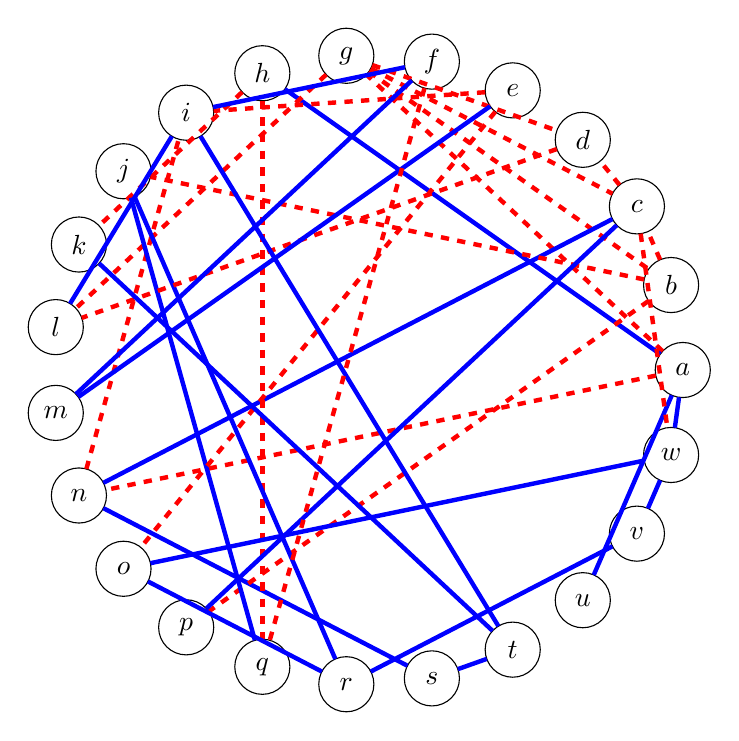
\begin{tikzpicture}[
          node distance=2cm, % Adjust as needed
          every node/.style={circle,draw,minimum size=0.7cm,inner sep=0,outer sep=0},
          blue edge/.style={blue, ultra thick},
          red edge/.style={red, ultra thick, dashed},
          xscale=4, % Adjust scaling as needed
          yscale=4,
        ]
        
        % Node positions
        \node (a) at (1.0,1.2957531388962193e-08) {$a$};
        \node (g) at (-0.06824243866721937,0.9976687496274143) {$g$};
        \node (n) at (-0.9172112817530316,-0.39840106602336356) {$n$};
        \node (u) at (0.6825530549588861,-0.7308360757333034) {$u$};
        \node (h) at (-0.3348795685115096,0.942260927854278) {$h$};
        \node (b) at (0.9629172685164649,0.2697967999020556) {$b$};
        \node (j) at (-0.7757112268798297,0.6310879676815739) {$j$};
        \node (p) at (-0.5766802328003474,-0.8169699724797971) {$p$};
        \node (c) at (0.8544194111719118,0.5195839500972502) {$c$};
        \node (d) at (0.6825531145635304,0.7308359824390775) {$d$};
        \node (w) at (0.9629173281211093,-0.2697965355684152) {$w$};
        \node (l) at (-0.9906859268916305,0.13616653994265754) {$l$};
        \node (e) at (0.4600650405102123,0.8878852201033856) {$e$};
        \node (o) at (-0.7757113460891185,-0.6310878821618667) {$o$};
        \node (i) at (-0.5766803520096362,0.8169698791855711) {$i$};
        \node (f) at (0.20345604935770417,0.9790840811114979) {$f$};
        \node (m) at (-0.9906859268916305,-0.13616669284152794) {$m$};
        \node (q) at (-0.33487953870918735,-0.9422609019392152) {$q$};
        \node (k) at (-0.9172112817530316,0.39840115154307076) {$k$};
        \node (t) at (0.46006495110324575,-0.8878852537929671) {$t$};
        \node (r) at (-0.06824237906257498,-0.9976687237123514) {$r$};
        \node (v) at (0.854419291962623,-0.5195841029961206) {$v$};
        \node (s) at (0.20345598975305978,-0.9790840551964352) {$s$};
        
        % Edges
        \draw[red edge] (a) -- (g);
        \draw[red edge] (a) -- (n);
        \draw[blue edge] (a) -- (u);
        \draw[blue edge] (a) -- (h);
        \draw[blue edge] (a) -- (w);
        \draw[red edge] (g) -- (b);
        \draw[red edge] (g) -- (c);
        \draw[red edge] (g) -- (d);
        \draw[red edge] (g) -- (l);
        \draw[blue edge] (n) -- (c);
        \draw[red edge] (n) -- (i);
        \draw[blue edge] (n) -- (s);
        \draw[red edge] (h) -- (k);
        \draw[red edge] (h) -- (q);
        \draw[red edge] (b) -- (j);
        \draw[red edge] (b) -- (p);
        \draw[red edge] (b) -- (c);
        \draw[blue edge] (j) -- (r);
        \draw[blue edge] (j) -- (q);
        \draw[blue edge] (p) -- (c);
        \draw[red edge] (c) -- (d);
        \draw[red edge] (c) -- (w);
        \draw[red edge] (d) -- (l);
        \draw[blue edge] (w) -- (o);
        \draw[blue edge] (w) -- (v);
        \draw[blue edge] (l) -- (i);
        \draw[red edge] (e) -- (o);
        \draw[red edge] (e) -- (i);
        \draw[blue edge] (e) -- (m);
        \draw[blue edge] (o) -- (r);
        \draw[blue edge] (i) -- (f);
        \draw[blue edge] (i) -- (t);
        \draw[blue edge] (f) -- (m);
        \draw[red edge] (f) -- (q);
        \draw[blue edge] (k) -- (t);
        \draw[blue edge] (t) -- (s);
        \draw[blue edge] (r) -- (v);
        
        \end{tikzpicture}
    }
    \resizebox{.24\textwidth}{!}{%
        % reconstruction 2
        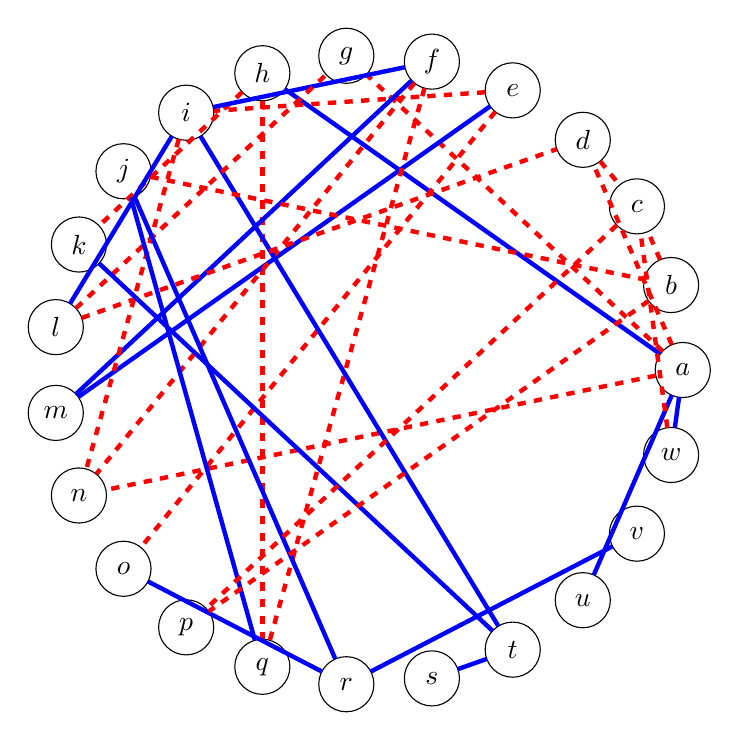
\begin{tikzpicture}[
          node distance=2cm, % Adjust as needed
          every node/.style={circle,draw,minimum size=0.7cm,inner sep=0,outer sep=0},
          blue edge/.style={blue, ultra thick},
          red edge/.style={red, ultra thick, dashed},
          xscale=4, % Adjust scaling as needed
          yscale=4,
        ]
        
        % Node positions
        \node (a) at (1.0,1.2957531388962193e-08) {$a$};
        \node (h) at (-0.3348795685115096,0.942260927854278) {$h$};
        \node (u) at (0.6825530549588861,-0.7308360757333034) {$u$};
        \node (w) at (0.9629173281211093,-0.2697965355684152) {$w$};
        \node (e) at (0.4600650405102123,0.8878852201033856) {$e$};
        \node (m) at (-0.9906859268916305,-0.13616669284152794) {$m$};
        \node (f) at (0.20345604935770417,0.9790840811114979) {$f$};
        \node (i) at (-0.5766803520096362,0.8169698791855711) {$i$};
        \node (l) at (-0.9906859268916305,0.13616653994265754) {$l$};
        \node (t) at (0.46006495110324575,-0.8878852537929671) {$t$};
        \node (j) at (-0.7757112268798297,0.6310879676815739) {$j$};
        \node (q) at (-0.33487953870918735,-0.9422609019392152) {$q$};
        \node (r) at (-0.06824237906257498,-0.9976687237123514) {$r$};
        \node (k) at (-0.9172112817530316,0.39840115154307076) {$k$};
        \node (o) at (-0.7757113460891185,-0.6310878821618667) {$o$};
        \node (v) at (0.854419291962623,-0.5195841029961206) {$v$};
        \node (s) at (0.20345598975305978,-0.9790840551964352) {$s$};
        \node (d) at (0.6825531145635304,0.7308359824390775) {$d$};
        \node (g) at (-0.06824243866721937,0.9976687496274143) {$g$};
        \node (n) at (-0.9172112817530316,-0.39840106602336356) {$n$};
        \node (b) at (0.9629172685164649,0.2697967999020556) {$b$};
        \node (c) at (0.8544194111719118,0.5195839500972502) {$c$};
        \node (p) at (-0.5766802328003474,-0.8169699724797971) {$p$};
        
        % Edges
        \draw[blue edge] (a) -- (h);
        \draw[blue edge] (a) -- (u);
        \draw[blue edge] (a) -- (w);
        \draw[red edge] (a) -- (d);
        \draw[red edge] (a) -- (g);
        \draw[red edge] (a) -- (n);
        \draw[red edge] (h) -- (k);
        \draw[red edge] (h) -- (q);
        \draw[red edge] (w) -- (c);
        \draw[blue edge] (e) -- (m);
        \draw[red edge] (e) -- (i);
        \draw[red edge] (e) -- (o);
        \draw[blue edge] (m) -- (f);
        \draw[blue edge] (f) -- (i);
        \draw[red edge] (f) -- (n);
        \draw[red edge] (f) -- (q);
        \draw[blue edge] (i) -- (l);
        \draw[blue edge] (i) -- (t);
        \draw[red edge] (i) -- (n);
        \draw[red edge] (l) -- (d);
        \draw[red edge] (l) -- (g);
        \draw[blue edge] (t) -- (k);
        \draw[blue edge] (t) -- (s);
        \draw[blue edge] (j) -- (q);
        \draw[blue edge] (j) -- (r);
        \draw[red edge] (j) -- (b);
        \draw[blue edge] (r) -- (o);
        \draw[blue edge] (r) -- (v);
        \draw[red edge] (d) -- (c);
        \draw[red edge] (b) -- (c);
        \draw[red edge] (b) -- (p);
        \draw[red edge] (c) -- (p);
        
        \end{tikzpicture}
    }
    \resizebox{.49\textwidth}{!}{%
        % true 2
        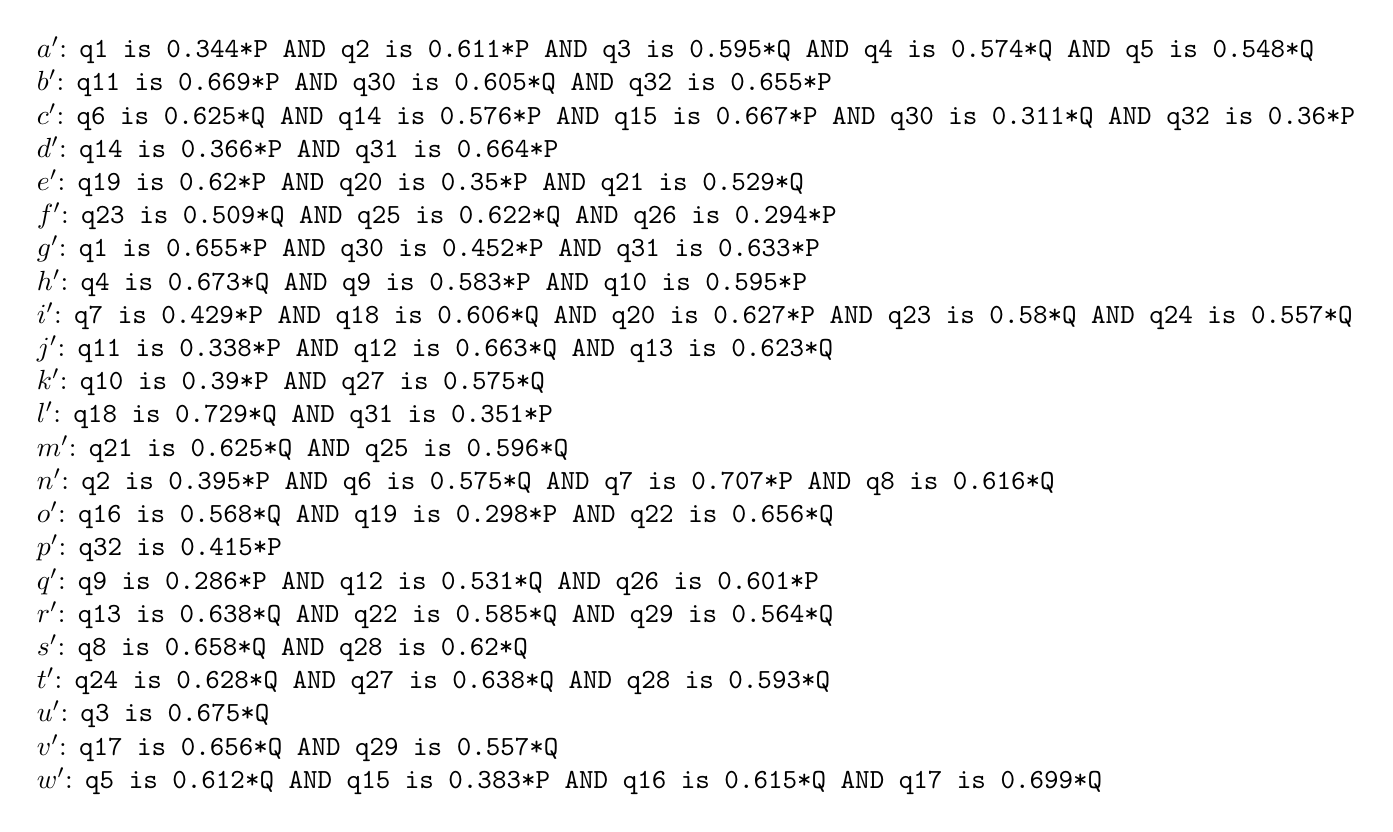
\begin{tikzpicture}[
          xscale=4, % Adjust scaling as needed
          yscale=4,
        ]
            \node[align=left] (a) at (0,0) {
                $a'$: \texttt{q1 is 0.344*P AND q2 is 0.611*P AND q3 is 0.595*Q AND q4 is 0.574*Q AND q5 is 0.548*Q} \\
                $b'$: \texttt{q11 is 0.669*P AND q30 is 0.605*Q AND q32 is 0.655*P} \\
                $c'$: \texttt{q6 is 0.625*Q AND q14 is 0.576*P AND q15 is 0.667*P AND q30 is 0.311*Q AND q32 is 0.36*P} \\
                $d'$: \texttt{q14 is 0.366*P AND q31 is 0.664*P} \\
                $e'$: \texttt{q19 is 0.62*P AND q20 is 0.35*P AND q21 is 0.529*Q} \\
                $f'$: \texttt{q23 is 0.509*Q AND q25 is 0.622*Q AND q26 is 0.294*P} \\
                $g'$: \texttt{q1 is 0.655*P AND q30 is 0.452*P AND q31 is 0.633*P} \\
                $h'$: \texttt{q4 is 0.673*Q AND q9 is 0.583*P AND q10 is 0.595*P} \\
                $i'$: \texttt{q7 is 0.429*P AND q18 is 0.606*Q AND q20 is 0.627*P AND q23 is 0.58*Q AND q24 is 0.557*Q} \\
                $j'$: \texttt{q11 is 0.338*P AND q12 is 0.663*Q AND q13 is 0.623*Q} \\
                $k'$: \texttt{q10 is 0.39*P AND q27 is 0.575*Q} \\
                $l'$: \texttt{q18 is 0.729*Q AND q31 is 0.351*P} \\
                $m'$: \texttt{q21 is 0.625*Q AND q25 is 0.596*Q} \\
                $n'$: \texttt{q2 is 0.395*P AND q6 is 0.575*Q AND q7 is 0.707*P AND q8 is 0.616*Q} \\
                $o'$: \texttt{q16 is 0.568*Q AND q19 is 0.298*P AND q22 is 0.656*Q} \\
                $p'$: \texttt{q32 is 0.415*P} \\
                $q'$: \texttt{q9 is 0.286*P AND q12 is 0.531*Q AND q26 is 0.601*P} \\
                $r'$: \texttt{q13 is 0.638*Q AND q22 is 0.585*Q AND q29 is 0.564*Q} \\
                $s'$: \texttt{q8 is 0.658*Q AND q28 is 0.62*Q} \\
                $t'$: \texttt{q24 is 0.628*Q AND q27 is 0.638*Q AND q28 is 0.593*Q} \\
                $u'$: \texttt{q3 is 0.675*Q} \\
                $v'$: \texttt{q17 is 0.656*Q AND q29 is 0.557*Q} \\
                $w'$: \texttt{q5 is 0.612*Q AND q15 is 0.383*P AND q16 is 0.615*Q AND q17 is 0.699*Q}
            };
        \end{tikzpicture}
    }
  \caption{
  Left: another coherence graph from our benchmark with edge density target $0.15$ (``sparse''). Center: \texttt{o1-mini} achieved good but imperfect ($F_1 = 0.96$: see vertices $c$, $d$, $g$, $n$, and $o$) reconstruction on this example under high uncertainty. Right: the modeling propositions incorporated high uncertainty.
}
  \label{fig:example2}
\end{figure}

% Applying the proposition generation algorithm described above 
This yields proposition sets involving a range of variable and property counts as enumerated in \S \ref{sec:graph_characteristics}. For each problem, we generate four additional sets of propositions. Three of these correspond to the noise regimes described above. We also generate a set of propositions where we add no noise (i.e., $p \leftarrow 1 * p$ and $\lnot p \leftarrow 0 * P$) in order to control for the presence of distractors in the evaluation.

Figure \ref{fig:example1} shows an example problem from the benchmark including a synthetic coherence graph with 21 nodes, propositions synthesized for the graph, and \texttt{o1-mini}'s perfect reconstruction of the input graph. Figure \ref{fig:example2} is similar, but the reconstruction is imperfect.


\subsection{\label{sec:prompts}Prompts}
We use a common prompt structure shown in \S \ref{sec:prompt_example} that a) establishes the consistency reasoning task, b) describes the variables and properties relevant for evaluating a set of propositions, c) establishes fuzzy membership thresholds for properties and d) embeds propositions for a given problem.


\section{\label{sec:results}Results}


\subsection{\label{sec:inference_results}LLMs successfully infer synthetic coherence graphs from a single prompt} 
Model performance varies considerably, with \texttt{o1-mini}, \texttt{claude-3.5-sonnet} and \texttt{QwQ-32B} outperforming the other models for both \texttt{sparse} and \texttt{dense} problems: see Figure \ref{fig:cohere_graphs}. 
 
\begin{figure}[htbp]
    \centering
    \includegraphics[width=1\linewidth, trim={0 8 0 0mm}, clip]{coherence_graphs_01312025.png}
        \caption{\texttt{o1-mini}, \texttt{claude-3.5-sonnet}, and \texttt{QwQ-32B} have high micro $F_1$ scores.}
    \label{fig:cohere_graphs}
\end{figure}

\subsection{\label{sec:uncertain_inference_results}LLMs successfully infer synthetic coherence graphs under uncertainty}
Table \ref{tab:graph_uncertainty_01312025} shows that introducing uncertainty does not degrade graph reconstruction fidelity. 

In Figure \ref{fig:uncertainty_examples}, we show how recursively passing an inferred uncertain coherence graph to \texttt{o1-mini} and prompting it to assign weights reflective of the level of uncertainty in property assignments can yield a weighted coherence graph with appropriate edge weights (less certain assignments yield smaller magnitude weights; more certain assignments yield larger magnitude weights).

\begin{figure}[htbp]
\centering
\vspace{-1cm}
\begin{minipage}{0.45\textwidth}
\centering
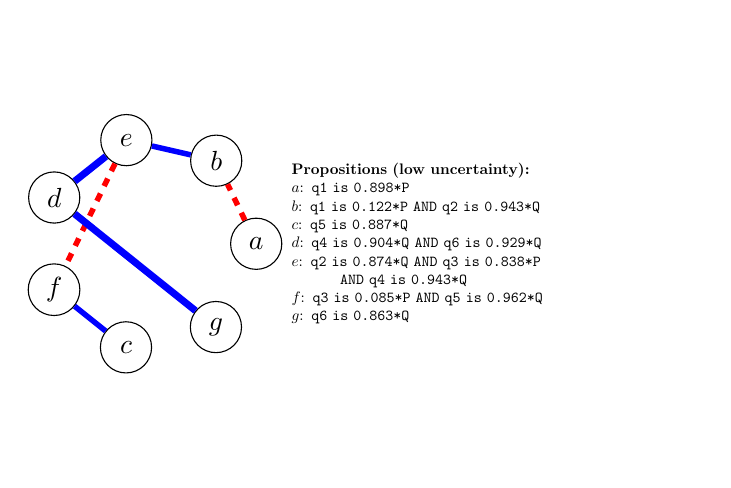
\begin{tikzpicture}[
  node distance=1cm,
  every node/.style={circle, draw, minimum size=.5cm, inner sep=0.1cm, align=center},
  positive edge/.style={blue, thick},
  negative edge/.style={red, thick, dashed},
  xscale=.45, % Adjust scaling as needed
  yscale=.45,
]

  % Nodes in a circle
  \node[draw,circle,fill=white,minimum size=6.5mm] (a) at (0:3) {$a$};
  \node[draw,circle,fill=white,minimum size=6.5mm] (b) at (51.4:3) {$b$};
  \node[draw,circle,fill=white,minimum size=6.5mm] (e) at (102.8:3) {$e$};
  \node[draw,circle,fill=white,minimum size=6.5mm] (d) at (154.2:3) {$d$};
  \node[draw,circle,fill=white,minimum size=6.5mm] (f) at (205.6:3) {$f$};
  \node[draw,circle,fill=white,minimum size=6.5mm] (c) at (257:3) {$c$};
  \node[draw,circle,fill=white,minimum size=6.5mm] (g) at (308.4:3) {$g$};

  % Edges with variable width based on weight
  \draw[negative edge, line width=0.7mm] (a) -- (b);
  \draw[positive edge, line width=0.7mm] (b) -- (e);
  \draw[positive edge, line width=0.9mm] (e) -- (d);
  \draw[negative edge, line width=0.7mm] (e) -- (f);
  \draw[positive edge, line width=0.9mm] (d) -- (g);
  \draw[positive edge, line width=0.7mm] (f) -- (c);

  % Propositions list
  \node[align=left] at (9.5, 0) [draw=none, text width=9cm, scale=0.55] {
    \textbf{Propositions (low \textbf{uncertainty}):} \\
    $a$: \texttt{q1 is 0.898*P} \\
    $b$: \texttt{q1 is 0.122*P AND q2 is 0.943*Q} \\
    $c$: \texttt{q5 is 0.887*Q} \\
    $d$: \texttt{q4 is 0.904*Q AND q6 is 0.929*Q} \\
    $e$: \texttt{q2 is 0.874*Q AND q3 is 0.838*P} \\ \hspace*{1cm} \texttt{AND q4 is 0.943*Q} \\
    $f$: \texttt{q3 is 0.085*P AND q5 is 0.962*Q} \\
    $g$: \texttt{q6 is 0.863*Q} \\
  };
\end{tikzpicture}
\end{minipage}
\quad \quad
\begin{minipage}{0.45\textwidth}
\centering
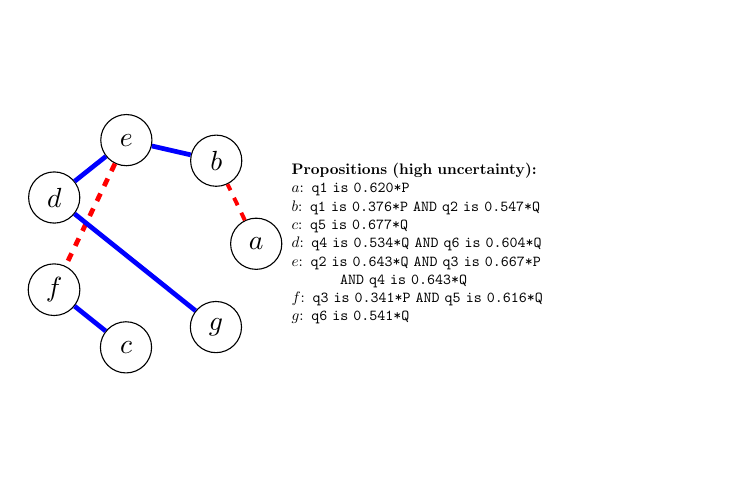
\begin{tikzpicture}[
  node distance=1cm,
  every node/.style={circle, draw, minimum size=.5cm, inner sep=0.1cm, align=center},
  positive edge/.style={blue, thick},
  negative edge/.style={red, thick, dashed},
  xscale=.45, % Adjust scaling as needed
  yscale=.45,
]

  % Nodes in a circle
  \node[draw,circle,fill=white,minimum size=6.5mm] (a) at (0:3) {$a$};
  \node[draw,circle,fill=white,minimum size=6.5mm] (b) at (51.4:3) {$b$};
  \node[draw,circle,fill=white,minimum size=6.5mm] (e) at (102.8:3) {$e$};
  \node[draw,circle,fill=white,minimum size=6.5mm] (d) at (154.2:3) {$d$};
  \node[draw,circle,fill=white,minimum size=6.5mm] (f) at (205.6:3) {$f$};
  \node[draw,circle,fill=white,minimum size=6.5mm] (c) at (257:3) {$c$};
  \node[draw,circle,fill=white,minimum size=6.5mm] (g) at (308.4:3) {$g$};

  % Edges with variable width based on weight
  \draw[negative edge, line width=0.5mm] (a) -- (b);
  \draw[positive edge, line width=0.6mm] (b) -- (e);
  \draw[positive edge, line width=0.6mm] (e) -- (d);
  \draw[negative edge, line width=0.6mm] (e) -- (f);
  \draw[positive edge, line width=0.6mm] (d) -- (g);
  \draw[positive edge, line width=0.6mm] (f) -- (c);

  % Propositions list
  \node[align=left] at (9.5, 0) [draw=none, text width=9cm, scale=0.55] {
\textbf{Propositions (high \textbf{uncertainty}):} \\
    $a$: \texttt{q1 is 0.620*P} \\
    $b$: \texttt{q1 is 0.376*P AND q2 is 0.547*Q} \\
    $c$: \texttt{q5 is 0.677*Q} \\
    $d$: \texttt{q4 is 0.534*Q AND q6 is 0.604*Q} \\
    $e$: \texttt{q2 is 0.643*Q AND q3 is 0.667*P} \\ \hspace*{1cm} \texttt{AND q4 is 0.643*Q} \\
    $f$: \texttt{q3 is 0.341*P AND q5 is 0.616*Q} \\
    $g$: \texttt{q6 is 0.541*Q} \\
  };
\end{tikzpicture}
\end{minipage}
\vspace{-1cm}
\caption{\texttt{o1-mini}-inferred weights have larger magnitude (indicated by edge thickness) when uncertainty is lower (as in the left panel). Both left and right panels reflect perfect reconstructions of the underlying graph.}
\label{fig:uncertainty_examples}
\end{figure}

% \begin{figure}[htbp]
% \centering
% \vspace{-1cm}
% \begin{minipage}{0.45\textwidth}
% \centering
% \begin{tikzpicture}[
%   node distance=1cm,
%   every node/.style={circle, draw, minimum size=.5cm, inner sep=0.1cm, align=center},
%   positive edge/.style={blue, thick},
%   negative edge/.style={red, thick, dashed},
%   xscale=.45, % Adjust scaling as needed
%   yscale=.45,
% ]

%   % Nodes in a circle
%   \node[draw,circle,fill=white,minimum size=6.5mm] (a) at (0:3) {$a$};
%   \node[draw,circle,fill=white,minimum size=6.5mm] (b) at (51.4:3) {$b$};
%   \node[draw,circle,fill=white,minimum size=6.5mm] (e) at (102.8:3) {$e$};
%   \node[draw,circle,fill=white,minimum size=6.5mm] (d) at (154.2:3) {$d$};
%   \node[draw,circle,fill=white,minimum size=6.5mm] (f) at (205.6:3) {$f$};
%   \node[draw,circle,fill=white,minimum size=6.5mm] (c) at (257:3) {$c$};
%   \node[draw,circle,fill=white,minimum size=6.5mm] (g) at (308.4:3) {$g$};

%   % Edges with variable width based on weight
%   \draw[negative edge, line width=0.7mm] (a) -- (b);
%   \draw[positive edge, line width=0.7mm] (b) -- (e);
%   \draw[positive edge, line width=0.9mm] (e) -- (d);
%   \draw[negative edge, line width=0.7mm] (e) -- (f);
%   \draw[positive edge, line width=0.9mm] (d) -- (g);
%   \draw[positive edge, line width=0.7mm] (f) -- (c);

%   % Propositions list
%   \node[align=left] at (9.5, 0) [draw=none, text width=9cm, scale=0.55] {
%     \textbf{Propositions (low \textbf{uncertainty}):} \\
%     $a$: $q_1$ is $0.898P$ \\
%     $b$: $q_1$ is $0.122P$ AND $q_2$ is $0.943Q$ \\
%     $c$: $q_5$ is $0.887Q$ \\
%     $d$: $q_4$ is $0.904Q$ AND $q_6$ is $0.929Q$ \\
%     $e$: $q_2$ is $0.874Q$ AND $q_3$ is $0.838P$ \\ \hspace*{1cm} AND $q_4$ is $0.943Q$ \\
%     $f$: $q_3$ is $0.085P$ AND $q_5$ is $0.962Q$ \\
%     $g$: $q_6$ is $0.863Q$ \\
%   };

% \end{tikzpicture}
% \end{minipage}
% \hfill
% \begin{minipage}{0.45\textwidth}
% \centering
% \begin{tikzpicture}[
%   node distance=1cm,
%   every node/.style={circle, draw, minimum size=.5cm, inner sep=0.1cm, align=center},
%   positive edge/.style={blue, thick},
%   negative edge/.style={red, thick, dashed},
%   xscale=.45, % Adjust scaling as needed
%   yscale=.45,
% ]

%   % Nodes in a circle
%   \node[draw,circle,fill=white,minimum size=6.5mm] (a) at (0:3) {$a$};
%   \node[draw,circle,fill=white,minimum size=6.5mm] (b) at (51.4:3) {$b$};
%   \node[draw,circle,fill=white,minimum size=6.5mm] (e) at (102.8:3) {$e$};
%   \node[draw,circle,fill=white,minimum size=6.5mm] (d) at (154.2:3) {$d$};
%   \node[draw,circle,fill=white,minimum size=6.5mm] (f) at (205.6:3) {$f$};
%   \node[draw,circle,fill=white,minimum size=6.5mm] (c) at (257:3) {$c$};
%   \node[draw,circle,fill=white,minimum size=6.5mm] (g) at (308.4:3) {$g$};

%   % Edges with variable width based on weight
%   \draw[negative edge, line width=0.5mm] (a) -- (b);
%   \draw[positive edge, line width=0.6mm] (b) -- (e);
%   \draw[positive edge, line width=0.6mm] (e) -- (d);
%   \draw[negative edge, line width=0.6mm] (e) -- (f);
%   \draw[positive edge, line width=0.6mm] (d) -- (g);
%   \draw[positive edge, line width=0.6mm] (f) -- (c);

%   % Propositions list
%   \node[align=left] at (9.5, 0) [draw=none, text width=9cm, scale=0.55] {
% \textbf{Propositions (high \textbf{uncertainty}):} \\
%     $a$: $q_1$ is $0.62P$ \\
%     $b$: $q_1$ is $0.376P$ AND $q_2$ is $0.547Q$ \\
%     $c$: $q_5$ is $0.677Q$ \\
%     $d$: $q_4$ is $0.534Q$ AND $q_6$ is $0.604Q$ \\
%     $e$: $q_2$ is $0.643Q$ AND $q_3$ is $0.667P$ \\ \hspace*{1cm} AND $q_4$ is $0.643Q$ \\
%     $f$: $q_3$ is $0.341P$ AND $q_5$ is $0.616Q$ \\
%     $g$: $q_6$ is $0.541Q$ \\
%   };
% \end{tikzpicture}
% \end{minipage}
% \vspace{-1cm}
% \caption{\texttt{o1-mini}-inferred weights have larger magnitude (indicated by edge thickness) when uncertainty is lower (as in the left panel). Both left and right panels reflect perfect reconstructions of the underlying graph.}
% \label{fig:uncertainty_examples}
% \end{figure}

\subsection{Minor post-processing is sometimes necessary to handle obvious reconstruction errors}
We noted four general types of reconstruction errors. First, some reconstructed graphs do not include a given proposition seen in the prompt. We observed this sporadically in all models. Second, we noticed some instances with Gemini models where the reconstructed graph contains nodes named, for instance, "Proposition(a)" instead of a or "(a)" instead of a. We noticed instances where \texttt{QwQ} incorrectly capitalized proposition names, for instance, substituting "A" for "a". We correct these first three error types in post-processing before evaluation.

Finally, we observed that some models hallucinate extra propositions in the reconstructed graph. Out of 608 inference attempts, \texttt{gemini-2.0-flash-exp} hallucinates on 10 inference attempts, \texttt{gpt-4o} on 5, \texttt{gemini-1.5-pro} on 4, and \texttt{Sky-T1-32B} on 1. We do not correct this type of error with post-processing; we instead eliminate these inference attempts from evaluation for these models since these hallucinations can be easily detected at runtime.

\begin{table}[h]
\centering
\small
%\begin{tabularx}{\textwidth}{XX|XXXXX}
\begin{tabular}{l l | l l l l l}
%\toprule
\hline
\textbf{model} & \textbf{sparsity} & \textbf{base case} & \textbf{zero unc.} & \textbf{low unc.} & \textbf{med unc.} & \textbf{high unc.} \\
%\midrule
\hline
\textbf{o1-mini} & \textbf{sparse} & 0.90 $\pm$ 0.17 & 0.89 $\pm$ 0.16 & 0.89 $\pm$ 0.15 & 0.89 $\pm$ 0.15 & 0.90 $\pm$ 0.16 \\
                 & \textbf{dense} & 0.69 $\pm$ 0.18 & 0.65 $\pm$ 0.19 & 0.63 $\pm$ 0.17 & 0.67 $\pm$ 0.18 & 0.68 $\pm$ 0.18 \\
\addlinespace
\textbf{Gemini 1.5} & \textbf{sparse} & 0.73 $\pm$ 0.22 & 0.74 $\pm$ 0.24 & 0.78 $\pm$ 0.18 & 0.82 $\pm$ 0.15 & 0.82 $\pm$ 0.15 \\
                        & \textbf{dense} & 0.49 $\pm$ 0.19 & 0.48 $\pm$ 0.19 & 0.46 $\pm$ 0.19 & 0.52 $\pm$ 0.18 & 0.52 $\pm$ 0.16 \\
\addlinespace
\textbf{Gemini 2.0} & \textbf{sparse} & 0.73 $\pm$ 0.24 & 0.68 $\pm$ 0.25 & 0.71 $\pm$ 0.25 & 0.73 $\pm$ 0.23 & 0.71 $\pm$ 0.27 \\
                              & \textbf{dense} & 0.49 $\pm$ 0.19 & 0.43 $\pm$ 0.16 & 0.44 $\pm$ 0.18 & 0.48 $\pm$ 0.17 & 0.49 $\pm$ 0.15 \\
\addlinespace
\textbf{GPT-4o} & \textbf{sparse} & 0.76 $\pm$ 0.20 & 0.77 $\pm$ 0.18 & 0.77 $\pm$ 0.22 & 0.76 $\pm$ 0.19 & 0.76 $\pm$ 0.18 \\
                & \textbf{dense} & 0.50 $\pm$ 0.19 & 0.47 $\pm$ 0.18 & 0.44 $\pm$ 0.19 & 0.50 $\pm$ 0.22 & 0.48 $\pm$ 0.19 \\
\addlinespace
\textbf{Phi-4} & \textbf{sparse} & 0.46 $\pm$ 0.32 & 0.38 $\pm$ 0.33 & 0.36 $\pm$ 0.30 & 0.35 $\pm$ 0.31 & 0.36 $\pm$ 0.28 \\
                         & \textbf{dense} & 0.40 $\pm$ 0.21 & 0.40 $\pm$ 0.20 & 0.38 $\pm$ 0.20 & 0.42 $\pm$ 0.21 & 0.43 $\pm$ 0.20 \\
\addlinespace
\textbf{Claude 3.5} & \textbf{sparse} & 0.90 $\pm$ 0.14 & 0.90 $\pm$ 0.14 & 0.89 $\pm$ 0.15 & 0.90 $\pm$ 0.14 & 0.90 $\pm$ 0.13 \\
                                    & \textbf{dense} & 0.60 $\pm$ 0.14 & 0.59 $\pm$ 0.14 & 0.58 $\pm$ 0.14 & 0.60 $\pm$ 0.15 & 0.58 $\pm$ 0.16 \\
\addlinespace
\textbf{Llama 3.3} & \textbf{sparse} & 0.53 $\pm$ 0.28 & 0.51 $\pm$ 0.27 & 0.55 $\pm$ 0.24 & 0.61 $\pm$ 0.25 & 0.50 $\pm$ 0.28 \\
                                           & \textbf{dense} & 0.41 $\pm$ 0.18 & 0.45 $\pm$ 0.19 & 0.40 $\pm$ 0.18 & 0.43 $\pm$ 0.17 & 0.40 $\pm$ 0.18 \\
\addlinespace
\textbf{QwQ} & \textbf{sparse} & 0.92 $\pm$ 0.12 & 0.90 $\pm$ 0.15 & 0.91 $\pm$ 0.13 & 0.92 $\pm$ 0.13 & 0.92 $\pm$ 0.13 \\
                              & \textbf{dense} & 0.62 $\pm$ 0.20 & 0.59 $\pm$ 0.18 & 0.59 $\pm$ 0.21 & 0.61 $\pm$ 0.22 & 0.60 $\pm$ 0.21 \\
\addlinespace
\textbf{Sky-T1} & \textbf{sparse} & 0.78 $\pm$ 0.20 & 0.67 $\pm$ 0.27 & 0.61 $\pm$ 0.32 & 0.67 $\pm$ 0.27 & 0.71 $\pm$ 0.26 \\
                                       & \textbf{dense} & 0.43 $\pm$ 0.18 & 0.40 $\pm$ 0.19 & 0.41 $\pm$ 0.19 & 0.42 $\pm$ 0.20 & 0.41 $\pm$ 0.19 \\
%\bottomrule
\hline
%\end{tabularx}
\end{tabular}
\caption{LLMs successfully infer synthetic coherence graphs under uncertainty (unc).}
\label{tab:graph_uncertainty_01312025}
\end{table}


\section{\label{sec:conclusion}Conclusion}

CDI provides a good model for many forms of cognition, including perception and planning. Combining CDI with consistency evaluations by neural models may lead to advancements in the state of the art in these domains. Moreover, our results indicate that it is now feasible to computationally instantiate a coherence theory of truth \citep{sep-truth-coherence}. By hard-coding conclusively established propositions, this theory can be anchored in a correspondence theory of truth \citep{sep-truth-correspondence}. 


\section*{Acknowledgments}
Both authors thank Tejas Patel and Jim Simpson for useful exchanges, and Alexander Medeiros and Alberto Tolentino for software engineering and infrastructure support. SH also thanks George Cybenko, Neil Gerr, Ludmilla Huntsman, Rob Johnston, Michael Robinson, Benjamin Wittes, and Levent Yilmaz for useful exchanges. 
This research was developed with funding from the Defense Advanced Research Projects Agency (DARPA). The views, opinions and/or findings expressed are those of the author(s) and should not be interpreted as representing the official views or policies of the Department of Defense or the U.S. Government. Distribution Statement “A” (Approved for Public Release, Distribution Unlimited).


% \section*{Ethics Statement}
% \steve{No killer robots were harmed in the course of this research.}


\bibliography{benchmarkingCoherenceBib}


\appendix


\section{\label{sec:computation}Coherence can be computed in different ways}


\subsection{\label{sec:computationClassical}Classical coherence is equivalent to 2-MAX-XORSAT and to sparse approximation for 2-XORSAT}

There are a number of algorithms for computing coherence classically. Besides a brute force solution to the MAX-CUT problem for a coherence graph $G_\sigma$, there are also greedy stochastic, simulated annealing, and semidefinite programming approximations \citep{thagard1998coherence,gartner2012approximation}. Historically, the dominant approach is a dynamical neural (``connectionist'') algorithm discussed in \citet{thagard2002coherence}. However, implementations are sufficiently outdated or hard to work with 
\footnote{See, e.g., \url{https://github.com/mars0i/popco}, \url{https://github.com/russellcameronthomas/JavaECHO_command_line}, \url{https://github.com/B-Sabev/ComputationalModelsOfCoherence}, \url{https://github.com/tjd/echo}, or \url{https://github.com/MaxRae/ConnectionistSudoku}. Even the two most recent of these have not been updated for six years as of this writing.}
that an adaptation based on an Ising model has recently been developed \citep{maier2023comparing}. 

We proceed to outline two computational perspectives on coherence that to our knowledge have not previously been considered explicitly, though the second was discussed at the level of prose in \citet{huntsman2024prospects}. Given a coherence graph $G_\sigma$, the consistency equation $\sigma(v,w) = 1$ corresponds to an equation of the form $x_v + x_w = 0$ over the Boolean field $\mathbb{F}_2$, and also to the propositional clause $v \iff w$. Meanwhile, the inconsistency equation $\sigma(v,w) = -1$ corresponds to $x_v + x_w = 1$, and also to the propositional clause $v \oplus w$, where $\oplus = \text{XOR}$. Therefore, we can repackage $G_\sigma$ into the linear equation $Bx = c$, where $B$ is the incidence matrix of $G_\sigma$, or equivalently the biadjacency matrix of the factor graph of the 2-XORSAT/2-Affine-SAT \citep{roy2006fault,mezard2009information} formula obtained from the clauses indicated just above. 

For example, the coherence graph in Figure \ref{fig:variables} corresponds to the linear equation
\begin{equation}
\begin{pmatrix}
1 & 1 & 0 & 0 & 0 \\
0 & 1 & 1 & 0 & 0 \\
0 & 1 & 0 & 1 & 0 \\
0 & 1 & 0 & 0 & 1 \\
0 & 0 & 1 & 1 & 0 \\
0 & 0 & 0 & 1 & 1 \\
1 & 0 & 0 & 0 & 1
\end{pmatrix} 
\begin{pmatrix}
x_a \\ x_b \\ x_c \\ x_d \\ x_e
\end{pmatrix} 
=
\begin{pmatrix}
1 \\ 0 \\ 1 \\ 0 \\ 0 \\ 1 \\ 0
\end{pmatrix} 
\nonumber
\end{equation}
and also to the propositional formula
$$(a \oplus b) \land (b \iff b) \land (b \oplus d) \land (b \iff e) \land (c \iff d) \land (d \oplus e) \land (e \iff a).$$
By using the identities $v \iff w \equiv (\lnot v \lor w) \land (v \lor \lnot w)$ and $v \oplus w \equiv (v \lor w) \land (\lnot v \lor \lnot w)$, we can transform this into a CNF-SAT formula.

Of course, in general the linear equation has no solution and the propositional formula is unsatisfiable. In the propositional context, the coherence computation corresponds to the MAX-2-XORSAT problem, which unsurprisingly reduces to MAX-CUT \citep{moore2011nature}. To our knowledge, the linear algebra formulation of coherence does not appear in the literature. 
\footnote{However, this formulation of the MAX-XORSAT problem is found in the literature on low-density generator matrix codes, where it is equivalent to performing source encoding \citep{wainwright2010lossy}.
}
The goal is to find a certain approximate solution to $Bx = c$, where again $B$ is the incidence matrix (over $\mathbb{F}_2$) of $G_\sigma$, $x$ is a vector of propositional truth values, and $c$ is a vector encoding $\sigma$. Specifically, we want to find the assignment $x$ that satisfies the most rows of the equation: this is equivalent to satisfying the most clauses, i.e., to solving MAX-(2-XOR)SAT all over again. In the language of sparse approximation, we want to solve $\arg \min_x \|Bx-c\|_0$ over $\mathbb{F}_2$, where the $L^0$ ``norm'' (i.e., the size of the support) is indicated.
\footnote{Note that i) over $\mathbb{F}_2$, the $L^0$ and $L^1$ norms are the same, but this offers no advantage; and ii) the usual problem of sparse approximation is of the form $\min_y \|y\|_0$ such that $b = Ay$. Our problem is not expressible in this way and it does not appear to be treated in the literature from the perspective of sparse approximation/optimization, cf. \citep{natarajan1995sparse}. 
}
We can write this as a more conventional-looking optimization with objective $\sum_j (-1)^{c_j + e_j^T B x}$ \citep{jordan2024optimization}. However, there is a more general formulation as an integer linear program \citep{vazirani2001approximation} whose relaxation is of substantial practical interest, as we shall discuss in the sequel.


\subsection{\label{sec:computationGeneral}A general approach: weighted MAX-SAT}

We sketch how to represent higher-order (in)consistency relationships such as trilemmas. A conceptually simple but computationally involved general approach is as follows:
\begin{itemize}
    \item for each ordered pair of dependent claims, rate the consistency of the second given the first, and associate this to a weight for an implication term;
    \item for each ordered triple of dependent claims, rate the consistency of the second and third given the first, and separately the consistency of the third given the first and second: associate these with corresponding implication terms;
    \item etc., truncating this hierarchy as desired/practical. 
\end{itemize}
Note that this requires a clique-finding algorithm such as that of \citet{chiba1985arboricity}, and that each unordered tuple corresponds to several ordered tuples, ensuring symmetry.

While this approach appears to adequately generalize the notion of a coherence graph into what amounts to a weighted \emph{simplicial complex}---i.e., a weighted hypergraph containing all sub-hyperedges \citep{rosiak2022sheaf}---it is not yet suitable for practical MAX-SAT solvers of any sort. These only address weighted CNF-SAT problems, while common translations into CNF-SAT do not preserve weights correctly. Therefore, applying a MAX-SAT solver would generally require (implementing and) applying a specialized transformation of the sort detailed in \citet{li2022clausal}, which to our knowledge has no public implementation.

Once a coherence problem is properly transformed into CNF-SAT, there is an interesting alternative to weighted MAX-SAT solvers. An efficient probabilistic algorithm for weighted MAX-SAT discussed in \cite{vazirani2001approximation} provides a natural probabilistic interpretation that is certain to be useful in many if not most practical situations. For example, a proposition with acceptance probability near 0.5 may indicate a need for---and even drive the collection of---additional data for incorporation into the relevant structure.

The general approach to representing and solving ``higher-order'' coherence problems outlined just above was suggested by \citet{huntsman2024prospects}, who were unaware of prior work on coherence \emph{per se}. The underlying motivation was that a \emph{sheaf} ought to represent consistency data. Briefly, a sheaf is comprised of data on open sets in a topological space that satisfy natural restriction---equivalently, gluing---axioms \citep{rosiak2022sheaf}. The connection to sheaves is that every logical clause in a CNF-SAT formula introduces a logical constraint that must be satisfied in order for the overall formula to be satisfied. In particular, adding clauses can never enlarge the solution space \citep{srinivas1993applications}.

It is not immediately clear how to adapt our approach for modeling coherence graphs to this more general setting. We leave this for future work.


\section{\label{sec:vincennes}A case study comparing human and LLM consistency ratings}

There is additional evidence that LLMs can reliably gauge propositional (in)consistency \citep{huntsman2024prospects,kumar2024nlp}. However, we are not aware of any assessment of performance relative to humans. Here, we outline a case study performed in summer 2024 in which \texttt{ChatGPT 4} demonstrated superhuman performance at gauging (in)consistency.

In \citet{thagard1992adversarial}, a coherence graph modeled a decision facing the captain of the cruiser USS \emph{Vincennes} on 3 July 1988: was radar track 4131 taking off from the Iranian civilian-military airfield at Bandar Abbas a civilian aircraft, or a hostile F-14 preparing to attack? The coherence graph included ``positive evidence'' propositions (labeled E*) copied almost verbatim from \S III.C.1.b of the investigation report \citep{fogarty1988formal} along with a few of their negations (labeled NE*) and hypothetical propositions that the track was attacking (labeled A*) or commercial (labeled C*). As is still common today for analyses using CDI, the edge set and weights (here, simply signs) were constructed by hand.

To focus on \texttt{ChatGPT 4}'s performance in evaluating (in)consistency, we considered the same edge set as the manually-constructed coherence graph, i.e., we neglected any considerations of dependence.
\begin{quote}
    It is important to note here that (the nontrivial connected component of) the coherence graph has $|V| = 21$ and $|E| = 36$, so its edge density is $36/210 = 0.17$. {\bf In other words, this example is in exactly the same regime as the larger and sparser benchmark graphs discussed in the main text.}
\end{quote}
For each edge, we asked \texttt{ChatGPT 4} to rate the consistency of the corresponding pairs of propositions 10 times using a variant of the prompt in \citet{huntsman2024prospects} that included an extract from the executive summary of \citet{fogarty1988formal} as background information. The results are shown in Figures \ref{fig:vincennesGraphs} and \ref{fig:vincennesBars}. Supporting data and scripts are in \citet{huntsman2025vincennes}.

\begin{figure}[htbp]
    \centering
    \includegraphics[width=.45\linewidth, trim={110 55 95 20mm}, clip]{VincennesGraphThagard20240422.png}
    \quad \quad
    \includegraphics[width=.45\linewidth, trim={110 55 95 20mm}, clip]{VincennesGraphChatGPT20240422.png}
    \caption{Left: A hand-crafted coherence graph from \citet{thagard1992adversarial}. {\color{blue}Blue} and {\color{red}red} respectively indicate {\color{blue}positive} and {\color{red}negative} edge weights. Right: A coherence graph with the same edges, but with weights given by rescaled median consistency ratings from \texttt{ChatGPT 4}. Thickness indicates the relative magnitude of weights.
}
    \label{fig:vincennesGraphs}
\end{figure}

\begin{figure}[htbp]
    \centering
    \includegraphics[width=1\linewidth]{VincennesRatings20250122.png}
    \caption{{\color{blue}Rescaled median consistency ratings by \texttt{ChatGPT 4}} \emph{versus} {\color{red}hand-crafted consistency ratings from \citet{thagard1992adversarial}}.
}
    \label{fig:vincennesBars}
\end{figure}

A bit of introspection and common sense reveals that for the largest discrepancies between the median LLM rating and the human rating, the median LLM rating is more reasonable in each event. Consider the four largest discrepancies, listed in order of their appearance in Figure \ref{fig:vincennesBars}:
\begin{itemize}
    \setlength{\itemindent}{.25in}
    \item[A2-C2:] These are obviously consistent, so \texttt{ChatGPT 4}'s rating is better than the rating in \citet{thagard1992adversarial}.
    \begin{itemize}
        \item A2 is ``Track 4131 was an F-14.''
        \item C2 is ``Track 4131 was taking off.''
    \end{itemize}
    \item[A3-E3:] Examination of outputs shows that \texttt{ChatGPT 4} considered plausible technical failures and misunderstandings. In light of this, it is fair to conclude that \texttt{ChatGPT 4}'s rating is better than the rating in \citet{thagard1992adversarial}.
    \begin{itemize}
        \item A3 is ``Track 4131 intended to attack.''
        \item C3 is ``Track 4131 was not responding to verbal warnings over [air distress frequencies].''
    \end{itemize}
    \item[A3-C2:] Both A3 and C2 are listed above. These are obviously consistent, so \texttt{ChatGPT 4}'s rating is better than the rating in \citet{thagard1992adversarial}.
    \item[E12-C1:] Examination of outputs shows that \texttt{ChatGPT 4} considered navigation and communications emissions of commercial airliners. In light of this, it is fair to conclude that \texttt{ChatGPT 4}'s rating is better than the rating in \citet{thagard1992adversarial}.
    \begin{itemize}
        \item E12 is ``No [electronic emissions were reported] from track 4131, however, F-14s can fly [without electronic emissions].''
        \item C1 is ``Track 4131 was a commercial airliner.''
    \end{itemize}
\end{itemize}

To summarize, \texttt{ChatGPT 4} demonstrated superhuman performance at gauging the (in)consistency of propositions. 


\section{\label{sec:anova} ANOVA for micro $F_1$}

The two-way ANOVA for micro $F_1$ in Table \ref{tab:anova} shows significant effects.
% Requires: \usepackage{array}

\begin{table}[h]
    \centering
    \begin{tabular}{lrrrr}
        \toprule
        & \textbf{SS} & \textbf{DF} & \textbf{F} & $\textbf{p-value}$ \\
        \midrule
        \textbf{Model} & 9.69 & 8.0 & 29.62 & $<0.001$  \\
        \textbf{Sparsity} & 9.35 & 1.0 &228.51 & $<0.001$  \\
        \textbf{Model $\times$ sparsity} & 1.30 & 8.0 & 3.97 & $<0.001$  \\
        \textbf{Error} & 27.77 & 679.0 & \texttt{NaN} & \texttt{NaN} \\
        \bottomrule
    \end{tabular}
    \caption{A two-way ANOVA shows significance for model, sparsity, and their interaction.}
    \label{tab:anova}
\end{table}


\section{\label{sec:construction} Benchmark generation parameters can be altered to synthesize problem sets with desired characteristics} 

Figure \ref{fig:variables_and_properties} demonstrates how benchmark generation parameters lead to increasing numbers of variables in the resulting synthetic problem sets as graph sizes increase. The top row shows data for small graphs (5-11 propositions), middle row: medium graphs (13-17 propositions), bottom row: large graphs (19-23 propositions). In general, the \texttt{degenerate} edge clique processing method and the \texttt{partition} method (first and third subcolumns in each panel) lead to more variables and fewer properties than the \texttt{percolation} method (middle column of each panel). 

\begin{figure}[htbp]
    \centering
    \includegraphics[width=1\linewidth]{combined_pseudocolor.png}
    \caption{Figure \ref{fig:variables_and_properties} Changing benchmark generation parameters leads to increasing numbers of variables in the resulting synthetic problem sets as graph sizes increase. Top row: small graphs (5-11 propositions). Middle row: medium graphs (13-17 propositions). Bottom row: large graphs (19-23 props). In general, the \texttt{degenerate} edge clique processing method and the \texttt{partition} method (first and third subcolumns in each panel) lead to more variables and fewer properties than the \texttt{percolation} method (middle column of each panel).
} 
    \label{fig:variables_and_properties}
\end{figure}


\section{\label{sec:cross_encoders}Inferring logical entailment with \texttt{ModernBERT} fine-tuned for NLI}

 We performed a preliminary experiment to test whether we could directly identify either a) relevance (defined as two propositions sharing a single variable) or b) consistency directly from white box LLM embeddings or from a number of simple quantifications of inter-token attention in the models' attention mechanisms. While these experiments showed a consistently high error rate (suggesting the need for a more sophisticated mechanistic interpretabilty study along the lines described by \citealt{nanda2023progress}) we report the best results, which 
 came from using a small BERT model (\texttt{ModernBERT} fine-tuned to infer entailment relations between propositions \citep{sileo-2024-tasksource, reimers2019sentencebertsentenceembeddingsusing}. 
 
 Using propositions in the simplified natural language grammar of our benchmark shows accurate entailment inferences along the diagonal (left figure), but multiple errors in off-diagonal relations (e.g., inferring a contradiction in (2,4) between "$q_2$ is !P" and "$q_4$ is !P", among others). However, rewriting propositions more formally (right) shows that \texttt{ModernBERT} is able to perfectly infer consistency relations among these propositions.  

Our tests to extract logical relations directly from attention encodings included estimating e.g., mean or median inter-token attention at the first layer, last layer, or across all layers for \texttt{QwQ-32B} (the most performant open source LLM for our purposes) using benchmark propositions and propositions rewritten in propositional logic. We also tested applying regression to correct positional and autoregressive attention effects. These experiments were inconclusive, suggesting that more complex statistical measures might be needed to identify reasoning mechanisms in white box models.
 

\begin{figure}[htbp]
    \centering
\includegraphics[width=1\linewidth]{coherence_graph_nli.png}
      \caption{Pairwise natural language inference using \texttt{ModernBERT} for propositions of a simple one property problem shows errors on benchmark propositions (left) but perfect accuracy with propositions transformed to propositional logic (right).}
    \label{fig:v}
\end{figure}


\section{\label{sec:graph_characteristics} Characteristics of synthetic coherence graphs included in our benchmark experiment}

In Table \ref{tab:graph_characteristics}, we show that our experiment includes coherence graphs ranging in size from 5 to 23 propositions. We note that our requirement that all synthetic coherence graphs be connected makes harder to meet the desired sparsity (\texttt{sparse} and \texttt{dense} corresponding to target densities of 0.15 and 0.75 respectively) levels for smaller graphs (5-11 propositions).


\begin{table}[htbp]
    \centering
    \small
    \begin{tabular}{cc|c|c|c|c|c}
        \toprule
        \textbf{n propositions} & \textbf{sparsity} & \textbf{n variables} & \textbf{n properties} & \textbf{edges} & \textbf{density} & \textbf{problem} \\
        & & median & median & median & mean & count \\
        % \hline
        \midrule
        5 & \textbf{sparse} & 4.0 & 1.5 & 4.0 & 0.400000 & 4 \\
          & \textbf{dense} & 3.0 & 2.0 & 7.0 & 0.700000 & 4 \\
        % \hline
        \addlinespace
        7 & \textbf{sparse} & 6.0 & 2.0 & 6.0 & 0.285714 & 4 \\
          & \textbf{dense} & 5.5 & 2.0 & 15.0 & 0.714286 & 4 \\
        % \hline
        \addlinespace
        9 & \textbf{sparse} & 8.0 & 2.0 & 8.0 & 0.222222 & 4 \\
          & \textbf{dense} & 6.5 & 2.0 & 27.0 & 0.750000 & 4 \\
        % \hline
        \addlinespace
        11 & \textbf{sparse} & 10.0 & 2.0 & 10.0 & 0.181818 & 4 \\
           & \textbf{dense} & 9.5 & 3.0 & 41.0 & 0.745455 & 4 \\
        % \hline
        \addlinespace
        13 & \textbf{sparse} & 12.0 & 2.0 & 12.0 & 0.153846 & 4 \\
           & \textbf{dense} & 13.5 & 2.0 & 58.0 & 0.743590 & 4 \\
        % \hline
        \addlinespace
        15 & \textbf{sparse} & 15.0 & 2.0 & 15.0 & 0.142857 & 4 \\
           & \textbf{dense} & 17.5 & 2.5 & 78.0 & 0.742857 & 4 \\
        % \hline
        \addlinespace
        17 & \textbf{sparse} & 19.0 & 2.0 & 20.0 & 0.147059 & 4 \\
           & \textbf{dense} & 23.0 & 2.5 & 102.0 & 0.750000 & 4 \\
        % \hline
        \addlinespace
        19 & \textbf{sparse} & 22.0 & 2.0 & 25.0 & 0.146199 & 4 \\
           & \textbf{dense} & 29.0 & 2.5 & 128.0 & 0.748538 & 4 \\
        % \hline
        \addlinespace
        21 & \textbf{sparse} & 27.0 & 2.0 & 31.0 & 0.147619 & 3 \\
           & \textbf{dense} & 42.0 & 2.0 & 157.0 & 0.747619 & 3 \\
        % \hline
        \addlinespace
        23 & \textbf{sparse} & 32.0 & 2.0 & 37.0 & 0.146245 & 3 \\
           & \textbf{dense} & 52.0 & 2.0 & 189.0 & 0.747036 & 3 \\
        \bottomrule
    \end{tabular}
    \caption{Our experimental benchmark includes 76 graphs (N=38 \texttt{sparse} and N=38 \texttt{dense}) ranging in size from 5 to 23 propositions.
    }
    \label{tab:graph_characteristics}
\end{table}


\section{\label{sec:prompt_example} Prompt template for global consistency inference under uncertainty}

For the input set of propositions, identify which propositions are logically consistent (i.e., can coexist without contradiction). Construct a networkx graph where inconsistent edges are weight 1 and consistent edges are weight 0. If two vertices do not involve the same variables, do not create an edge between them.

\

Return solely the edge list with proposition names for vertices. i.e., return responses
in this format:

[('b', 'c', 0),

('b', 'e', 0),

('c', 'd', 0),

('c', 'e', 0)]

\

Variables:

['$q_1$', '$q_2$', '$q_3$', '$q_4$']

\

A given variable can have these properties:

property P: P XOR !P 

property Q: Q XOR !Q 

property R: R XOR !R 

property S: S XOR !S 

\

A given property is assigned in a fuzzy manner: 

property 1: !P := $<$ 0.5P. P := $\geq$ 0.5P 

property 2: !Q := $<$ 0.5Q. Q := $\geq$ 0.5Q 

property 3: !R := $<$ 0.5R. R := $\geq$ 0.5R 

property 4: !S := $<$ 0.5S. S := $\geq$ 0.5S 

\

Input: 

['Proposition(a): "$q_1$ is !P"', 

'Proposition(b): "$q_2$ is !P"', 

'Proposition(c): "$q_1$ is P AND $q_2$ is P AND $q_3$ is P"', 

'Proposition(d): "$q_4$ is !P"', 

'Proposition(e): "$q_3$ is !P AND $q_4$ is P"']


\section{\label{sec:l1_norm_graph_anova} Fidelity of the reconstruction of the graph measured by the $L^1$ norm normalized by graph size}{

Figure \ref{fig:cohere_graphs_l1} shows that \texttt{o1-mini}, \texttt{claude-3.5-sonnet} and \texttt{QwQ-32B-Preview} out perform all other models on \texttt{sparse} problems if we characterize reconstruction error using the measure of adjacency matrix similarity described in \S \ref{sec:benchmark}.


\begin{figure}[htbp]
    \centering
    \includegraphics[width=1\linewidth]{coherence_graphs_l1_norm_01312025.png}
        \caption{\texttt{o1-mini}, \texttt{claude-3.5-sonnet}, and \texttt{QwQ-32B} have lower (higher fidelity) $L_1$ scores than other models.}
    \label{fig:cohere_graphs_l1}
\end{figure}


\end{document}
